\chapter{Anwendungen}

Die zuvor in Kapitel \ref{ch:theory} eingeführten Methoden werden nun durch drei verschiedene Szenarien ausprobiert und verglichen. Hierbei liegt der Fokus auf der Verwendung und Erprobung der \textsc{ESN}s. Da die klassischen Methoden der \textit{nächsten Nachbarn} und der \textit{radialen Basisfunktionen} bereits seit längerer Zeit bekannt sind und populäre Lösung solcher Problemfälle darstellen, dienen sie als Bezugsgröße.\\

Jedes der drei Szenarien wird sowohl auf ein \textit{Barkley}-System als auch auf ein System nach dem \textit{Mitchell-Schaeffer}-Modell angewendet. Diese Systeme bestehen aus $150$ Gitterpunkten und nutzen die zuvor beschriebenen Parameter. Für ihre Startverteilung werden die Felder der beiden Systemvariablen in $100$ Quadrate unterteilt, und diese mit Zufallswerten zwischen $0$ und $1$ initialisiert. Anschließend werden die Systeme über $2000$ Zeitschritte ($\widehat{=} 400.0$ Zeiteinheiten) simuliert um ein transientes Verhalten abzuwarten. Durch das weitere Simulieren der Systeme werden die Test und Trainingsdaten ermittelt. Dabei wird für das \textit{Barkley} eine Samplingzeit von $0.1$ und für das \textit{Mitchell-Schaeffer}-Modell von $1.0$ Zeiteinheiten benutzt.\\
 
Die erste Aufgabe besteht darin aus der Kenntnis einer der beiden Systemvariablen die andere Unbekannte zu ermitteln. Dabei wird die Spannungsvariable als Quelle genutzt. Dies ist in den zuvor eingeführten Modellen jeweils die Größe, welche den Diffusionsterm beinhaltet; also die $u$-Variable im \textit{Barkley}-Modell und die $v$-Variable im \textit{Mitchell-Schaeffer}-Modell.\\
Im zweiten Szenario werden die Techniken verwendet um aus Messdaten einer simulierten Fernfeldmessung der Spannungsvariable  diese wiederherzustellen. Diese Fernfeldmessung wird durch eine gaußsche Unschärfe simuliert.\\
Abschließend wird die Spannungsvariable der inneren Punkte eines Quadrates nur durch die Kenntnis der Randwerte des Systems vorhergesagt.\\

%TODO ADD SUBCHAPTER?
\section{Allgemeines Vorgehen}
\label{sc:experiments_general}
Das Ziel aller drei Aufgaben besteht jeweils darin ein zweidimensionales Feld vorherzusagen. Eine naheliegende Möglichkeit dies zu schaffen besteht darin wirklich den gesamten Inhalt des $150 \times 150$ Einheiten großen Feldes auf einmal vorherzusagen. Da dabei die Ausgabe der Vorhersage aus einem $22500$-dimensionalen Vektor besteht werden sehr viele Trainingsdaten benötigt, um genügend Informationen über eine solch hochdimensionale Ausgabe zu erhalten. Um dieses Problem zu umgehen wird stattdessen ein Verfahren benutzt, bei dem jeder Punkt einzeln vorhergesagt wird. Dies hat zudem den Vorteil, dass aus einer monströsen Vorhersage, welche mitunter viel Arbeitsspeicher verbrauchen würde, in viele kleine Vorhersagen aufteilt. Hierdurch sinkt der zur Berechnung benötigte Bedarf an Arbeitsspeicher drastisch.\\

Des Weiteren kann angenommen werden, dass die Dynamiken einen ausgeprägten lokalen Charakter besitzen, sodass zumindest bei den ersten beiden Aufgaben weit entfernte Punkte keinen unmittelbaren Einfluss auf die Vorhersage haben. Darauf basierend kann eine sogenannte \textit{Messsondentechnik} entwickelt und für diese genutzt werden. Hierbei werden nicht nur die Informationen an einem Punkt $(i, j)$ für die Vorhersage, sondern auch die benachbarten Punkte, welche in einem Quadrat um $(i, j)$ liegen, genutzt. Eine Veranschaulichung ist in \ref{fig:probe_illustration_no_gaps} zu finden. Die Größe des Quadrates wird durch den Parameter $\sigma$ bestimmt, und ergibt sich zu $\sigma^2$. Da direkt Nachbarn unter Umständen durch den geringen Abstand sehr ähnliche Informationen beinhalten können, wird zudem ein Parameter $\Delta \sigma$ eingeführt, welche den Abstand zweier benachbarter Punkte, deren Information simultan verwendet werden, angibt. Eine beispielhafte Darstellung hiervon ist für $\sigma = 5, \Delta \sigma=2$ in Abbildung \ref{fig:probe_illustration_gaps} dargestellt. Dabei werden nur die Zeitreihen der Gitterpunkte genutzt, welche dunkelgrau hinterlegt sind, und die hellgrauen Informationen verworfen. Die Parameter, welche für die ersten beiden Aufgaben überprüft werden, sind in Tabelle \ref{tab:probe_sigma_values} aufgelistet. Dabei ist anzumerken, dass die Diskretisierung des Diffusionstermes in den Differentialgleichungen einem Wert $\sigma=3$ entsprechen würde.\\
Durch dieses Vorgehen kann für jeden Gitterpunkt ein ${\left \lceil{\frac{\sigma}{\Delta \sigma}}\right \rceil}^2$-dimensionaler Eingabevektor erstellt und für die ersten beiden Vorhersage-Aufgaben genutzt werden.

\begin{table}[h]
\centering
\begin{tabular}{c||c|c|c|c|c|c|c|}
$\sigma$ & 1 & 3 & \multicolumn{2}{c|}{5} & \multicolumn{3}{c|}{7} \\
\hline
$\Delta \sigma$ & 1 & 1 & 1 & 2 & 1 & 2 & 3 \\
\end{tabular} 
\caption{In den ersten beiden Aufgaben verwendete Parameter $\sigma$ und $\Delta \sigma$ für die \textit{Messsondentechnik}.}
\label{tab:probe_sigma_values}
\end{table} 

\begin{figure}[h]
\centering
\begin{subfigure}{.5\textwidth}
  \centering
  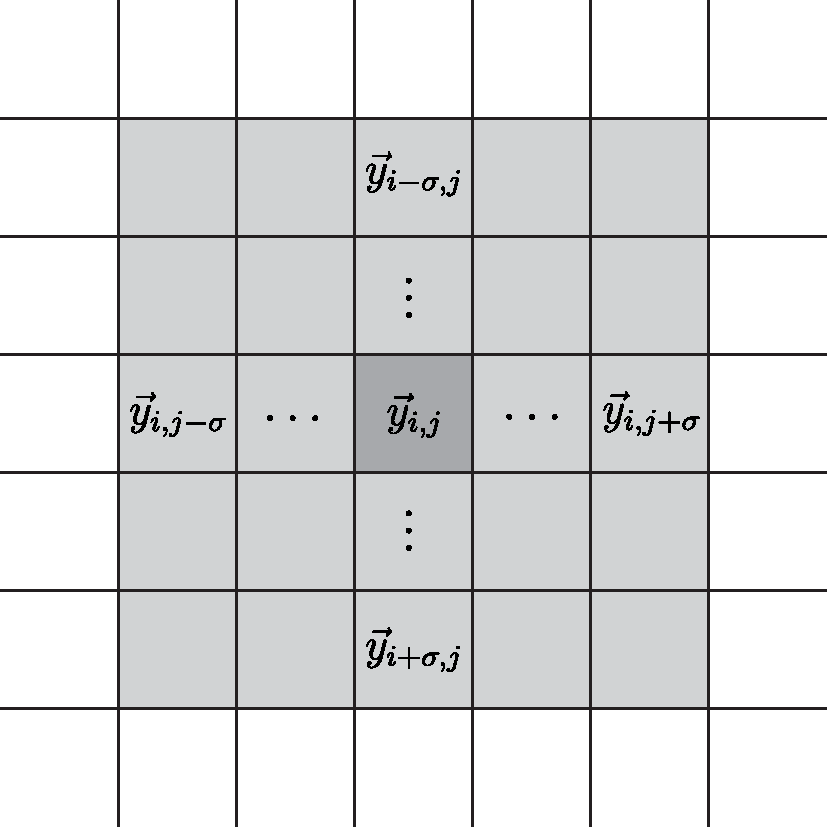
\includegraphics[width=.8\linewidth]{figures/illustrations/sigma_patches.pdf}
  \caption{Messsonde ohne Abstände zwischen\\den Messpunkten}
  \label{fig:probe_illustration_no_gaps}
\end{subfigure}%
\begin{subfigure}{.5\textwidth}
  \centering
  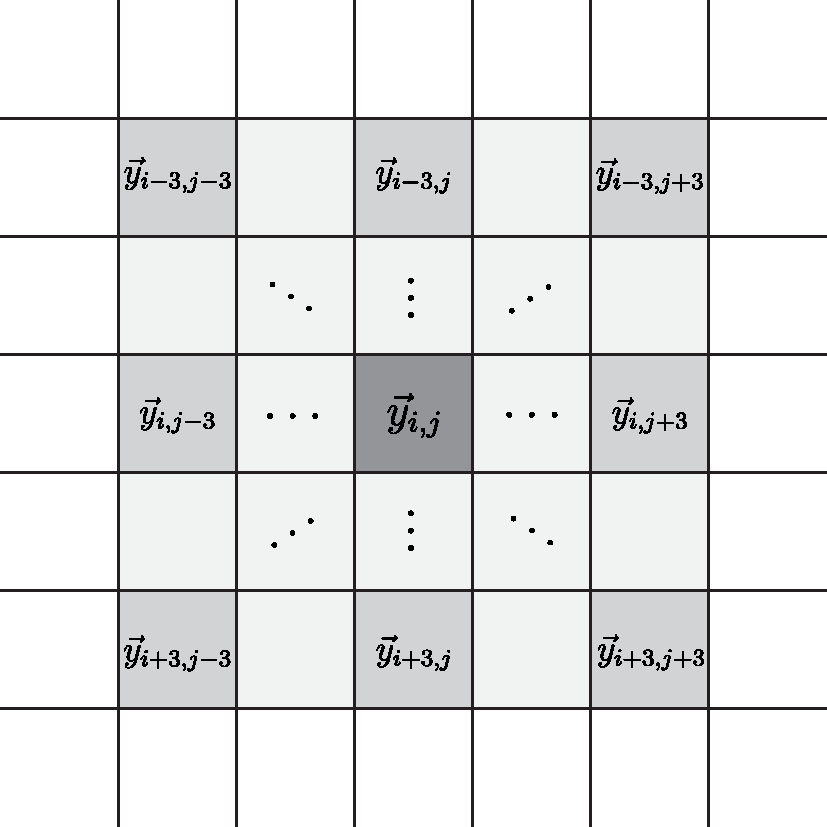
\includegraphics[width=.8\linewidth]{figures/illustrations/sigma_patches_gaps.pdf}
  \caption{Messonde mit einem Abstand von zwei Einheiten zwischen den Messpunkten}
  \label{fig:probe_illustration_gaps}
\end{subfigure}
\caption{Illustration der verwendeten \textit{Messsondentechnik}. Abbildung \ref{fig:probe_illustration_no_gaps} deutet an, wie aus einem $\sigma^2$ großem Quadrat um den eigentlichen Messpunkt Daten für die Vorhersage genutzt werden. Dagegen ist in Abbildung \ref{fig:probe_illustration_gaps} das Verfahren für $\sigma=5$ und $\Delta \sigma = 2$ dargestellt, sodass insgesamt die Information aus $9$ Punkten genutzt wird.}
\label{fig:probe_illustration}
\end{figure}

\subsection{Echo State Network}
\textit{Echo State Networks} besitzen viele verschiedene Hyperparameter, welche die Qualität der Vorhersage beeinflussen können. Dazu zählen nach \ref{sc:esn} die Reservoirgröße $N$, der Spektralradius $\rho$, die Verlustrate $\alpha$, die Amplitude der zufälligen Störung $\nu$, die Stärke der Regularisierung $\lambda$ und der Anteil der vorhandenen internen Verbindungen $\epsilon$. Da es zum aktuellen Zeitpunkt noch keinen zufriendenstellenden mathematischen Algorithmus für das das selbstständige optimale Einstellen eines \textsc{ESN}s gibt, müssen die Parameter manuell ermittelt werden. Hierfür wird in dieser Arbeit eine \textsc{GridSearch} benutzt. Bei diesem Verfahren wird der Hyperparameterraum in festgelegten Schritten abgetastet und die Leistung des somit entstehenden Netzwerke evaluiert und somit die besten Parameter ermittelt. Durch die hohe Anzahl der einstellbaren Hyperparameter und die nicht zu vernachlässigende Rechenzeit für das Trainieren und Evaluieren eines Netzwerkes, ist es nicht sinnvoll diese Suche für alle Datenpunkte gleichzeitig durchzuführen. Stattdessen wird zuerst unter der Annahme, dass die Dynamik sich lokal an allen Punkten ähnlich verhält, ein Punkt in der Mitte des Feldes ausgewählt, und nur versucht dieses einen einzelnen Punkt vorherzusagen. Diese Aufgabe kann deutlich schneller berechnet werden, sodass nun die optimalen Hyperparameter mit einer \textsc{GridSearch} gesucht werden können. Anschließend können die Hyperparameter des  zuvor ermittelten \textsc{ESN} für die Vorhersage aller Punkte genutzt werden.

\subsection{Klassische Methoden}
Die klassischen Methoden sind nicht von alleine aus in der Lage zeitlich ausgeprägte Dynamiken vorherzusagen, da den Methoden a priori keine Informationen über die vorherigen Zustände vorliegen. Um dieses Problem zu lösen können Verzögerungs-Koordinaten mittels der in Abschnitt \ref{sc:delay_reconstruction} beschriebenen \textit{Delay Reconstruction} für die in Abschnitt \ref{sc:experiments_general} beschriebenen Vektoren aufgestellt werden. Die über die Autokorrelation ermittelte zeitliche Verzögerung $\tau$ ist für beide Systeme in Tabelle \ref{tab:delay_reconstruction_tau} dargestellt.     

\begin{table}[h]
\centering
\begin{tabular}{|c|c|}
$\tau_{Barkley}$ & $\tau_{Mitchell-Schaeffer}$ \\ 
\hline 
\hline 
0.64 Zeiteinheiten & 2.38 Zeiteinheiten\\ 
\hline 
\end{tabular} 
\caption{Verwendete zeitliche Verzögerung $\tau$ für die \textit{Delay Reconstruction} für das \textit{Mitchell-Schaeffer}- und das \textit{Barkley}-Modell}
\label{tab:delay_reconstruction_tau}
\end{table} 

\section{Kreuz-Prädiktion}
\label{sec:exp_cross_pred}
Momentan ist es durch invitro Experimente bereits möglich die Ausbreitung der elektrischen Erregung auf der Oberfläche des Herzmuskels experimentell aufzuzeichnen. Nun stellt sich die Frage, ob anhand beispielsweise der Messung der Membramspannung weitere Variablen des Systems wie die Kalium-Konzentration oder ähnliches ermittelt werden kann. Diese Fragestellung wird in der ersten Aufgabe betrachtet. Es wird die Vorhersage von der Spannungsvariable auf die zweite Variable des jeweiligen Modells sowohl für das \textit{Barkley}- als auch für das \textit{Mitchell-Schaeffer}-Modell durchgeführt. Dabei wird zuerst die Nächste Nachbar Methode, anschließend die radialen Basisfunktionen und schlussendlich die \textit{ESN}s verwendet. Es werden sowohl die einzelnen Ergebnisse präsentiert als auch ein abschließender Vergleich durchgeführt.
 
\subsection{Nächste Nachbar Vorhersage}
Die Ergebnisse für die optimalen Hyperparameter des Modells $\delta \in \{3,4,5\}, k \in \{2, 3, 4, 5\}$ sind in Tabelle \ref{tab:exp_cross_nn_results} zu finden. Die Werte für $\sigma$ und $\Delta \sigma$ sind wie zuvor beschrieben variiert worden. Dabei sind sowohl die verwendeten Parameter als auch die erzielten Fehler MSE und NRMSE aufgelistet.
\begin{table}[h]
	\centering

	\begin{tabular}{ccc}
		\hline		
		\multicolumn{1}{c}{} & Barkley & Mitchell-Schaeffer \\ 
		\hline 
		\rule[-1ex]{0pt}{2.5ex} $\sigma$ & $1$ & $7$ \\ 
		\rule[-1ex]{0pt}{2.5ex} $\Delta \sigma$ & $1$ & $1$ \\ 
		\rule[-1ex]{0pt}{2.5ex} $\delta$ & $3$ & $3$ \\ 
		\rule[-1ex]{0pt}{2.5ex} k & $5$ & $5$ \\ 
		\rule[-1ex]{0pt}{2.5ex} Laufzeit [s] & $40$ & $5252$ \\ 
		\rule[-1ex]{0pt}{2.5ex} \textbf{MSE} & \textbf{0.00098} & \textbf{0.01891} \\ 
		\rule[-1ex]{0pt}{2.5ex} \textbf{NRMSE} & \textbf{0.1317} & \textbf{0.8795} \\ 
		\hline 
	\end{tabular} 

	\caption{Ermittelte Hyperparameter der nächsten Nachbar Vorhersage für das \textit{Mitchell-Schaeffer}- und das \textit{Barkley}-Modell, welche zu den geringsten Fehlern führen.}
\label{tab:exp_cross_nn_results}
\end{table} 

Dabei ist die stark unterschiedliche Laufzeit der beiden Vorhersagen auffällig. Dies lässt sich allerdings durch die verschiedenen Dimensionalitäten der Quellvariable erklären: Während beim \textit{Barkley}-Modell lediglich ein $3$-dimensionaler Vektor für die Vorhersage die besten Ergebnisse erzielt konnte beim \textit{Mitchell-Schaeffer}-Modell durch die Verwendung eines $147$-dimensionalen Quellvektors die besten Ergebnisse erzielt werden. Da, wie in Abschnitt \ref{sc:theory_nn} erwähnt, die benötigte Zeit für eine Vorhersage sehr stark mit der Dimension zunimmt, lässt sich somit der Anstieg von $40$ auf $5252$ Sekunden erklären.

Da eine Nächsten Nachbar Vorhersage nur anhand der in der Trainingsphase gesehenen Datenpunkte eine Vorhersage erstellt, ist anzunehmen, dass die Qualität dieser sehr stark von der Länge der Trainingsphase abhängt. Um dies zu untersuchen ist für die zuvor ermittelten Hyperparameter eine Vorhersage für verschiedene Trainingslängen $N_{Training}$ durchgeführt und die dabei auftretenden MSEs und die benötigte Laufzeit gemessen worden. Hierbei können zwei Effekte beobachtet werden. Bei der Betrachtung der grafischen Darstellung der benötigten Laufzeit in Abbildung \ref{fig:exp_cross_nn_trainlength_mse_time_barkley} für das \textit{Barkley}-Modell ist zu erkennen, dass sich der Zusammenhang zwischen $N_{Training}$ und der Laufzeit durch eine logarithmische Ausgleichskurve beschreiben lässt. Dies ist nach der theoretischen Betrachtung in \ref{sc:theory_nn} ein erwartetes Ergebnis. Der erzielte Fehler verhält sich dagegen anders und sinkt asymptotisch gegen eine untere Schranke ab. 

\begin{figure}[H]
	\centering
	\begin{subfigure}{.95\textwidth}
		\centering
		\hspace*{0.3cm}
		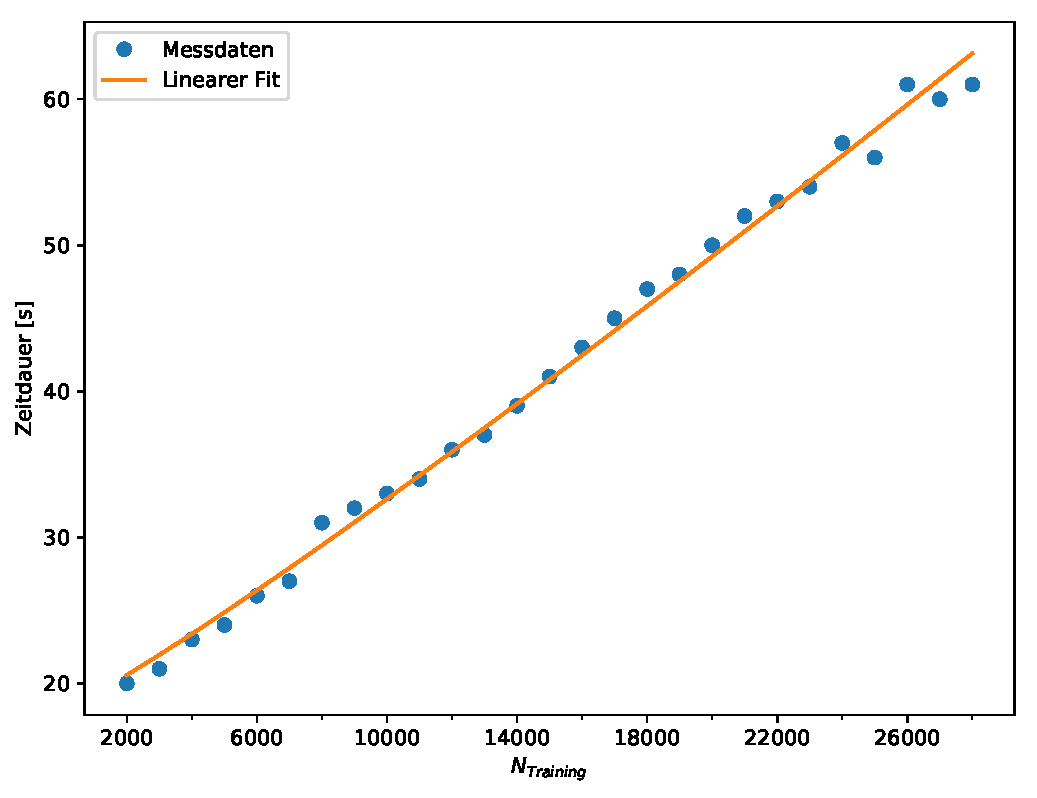
\includegraphics[width=.76\textwidth]{figures/results/cross_prediction/nn_trainlength_uv_time.pdf}
		\caption{Abhängigkeit der Laufzeit von $N_{Training}$.}
	\end{subfigure}%
	\\
	\begin{subfigure}{.95\textwidth}
		\centering
		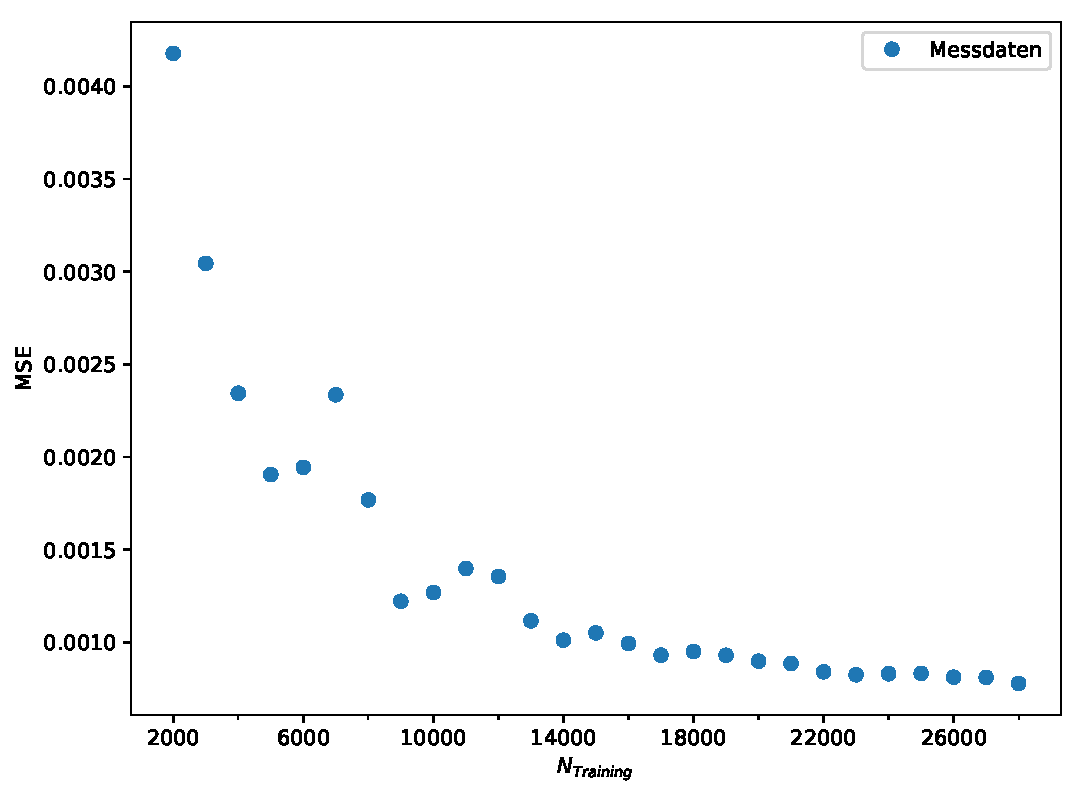
\includegraphics[width=.80\textwidth]{figures/results/cross_prediction/nn_trainlength_uv_mse.pdf}
		\caption{Abhängigkeit des \textit{MSE}s von $N_{Training}$.}
	\end{subfigure}%
	\caption{Darstellung der Abhängigkeit des benötigten Laufzeit (oben) und des MSE (unten) von der verwendeten Anzahl an Trainingsdaten $N_{Training}$ (unten) für das \textit{Barkley}-Modell bei der Verwendung einer nächsten Nachbar Vorhersage.}
	\label{fig:exp_cross_nn_trainlength_mse_time_barkley}
\end{figure}

Eine Analoge Darstellung für das \textit{Mitchell-Schaeffer}-Modell ist in \ref{fig:apx_exp_cross_nn_trainlength_mse_time_ms} zu finden. Anzumerken ist, dass die Sättigung des Fehlers im \textit{Barkley}-Modell schon ab etwa $N_{Training}=15000$ eintritt, doch beim \textit{Mitchell-Schaeffer}-Modell erst deutlich später. Dies ist ein Hinweis darauf, dass die Dynamiken im letzteren chaotischer und unregelmäßiger als bei ersten ablaufen. Zusammenfassend lässt sich somit die Wahl der Trainingslänge von $N_{Training} = 15000$ für alle Szenarien und alle drei Methoden damit begründen, dass man für die Nächste Nachbar Vorhersage, welche am empfindlichsten auf diese Länge reagiert, eine akzeptablen Kompromiss zwischen der Rechenzeit und der Genauigkeit erhält.

\FloatBarrier
\subsection{Radiale Basisfunktionen}
Bei der Verwendung radialer Basisfunktionen stellt zudem die Breite $\sigma_{RBF}$ der Gaußfunktionen als auch die Anzahl der Basisfunktionen $l$ einen wichtigen Parameter dar. Im Rahmen dieser Arbeit ist die Anzahl der Basisfunktionen auf $l=100$ festgelegt worden - diese Wahl wird im Folgenden weiter motiviert werden. Um die anderen Parameter zu finden, sind $\sigma$, $\Delta \sigma$ wie oben beschrieben, $\delta \in \{3,4,5\}$ und $\sigma_{RBF} \in \{0.5, 1.0, 3.0, 5.0, 7.0, 9.0\}$ variiert worden. In Tabelle \ref{tab:exp_cross_rbf_results} sind die dadurch gefundenen optimalen Parameter, die damit erreichten Fehler und die benötigte Laufzeit erneut für beide Modelle aufgelistet. Hierbei ist zu bemerken, dass die optimalen Werte für $\sigma$, $\Delta \sigma$ und $\delta$ mit denen für die NN-Vorhersage übereinstimmen. 

\begin{table}[h]
	\centering

	\begin{tabular}{ccc}
		\hline 			
		\multicolumn{1}{c}{} & Barkley & Mitchell-Schaeffer \\ 
		\hline 
		\rule[-1ex]{0pt}{2.5ex} $\sigma$ & $1$ & $7$ \\ 
		\rule[-1ex]{0pt}{2.5ex} $\Delta \sigma$ & $1$ & $1$ \\ 
		\rule[-1ex]{0pt}{2.5ex} $\delta$ & $3$ & $3$ \\ 
		\rule[-1ex]{0pt}{2.5ex} $\sigma_{RBF}$ & $0.5$ & $5$ \\ 
		\rule[-1ex]{0pt}{2.5ex} Laufzeit [s] & $1430$ & $1434$ \\ 
		\rule[-1ex]{0pt}{2.5ex} \textbf{MSE} & \textbf{0.01046} & \textbf{0.00948} \\ 
		\rule[-1ex]{0pt}{2.5ex} \textbf{NRMSE} & \textbf{0.1023} & \textbf{0.6228} \\ 
		\hline 
	\end{tabular} 
	\caption{Ermittelte Hyperparameter der radialen Basisfunktionen für das \textit{Mitchell-Schaeffer}- und das \textit{Barkley}-Modell, welche zu den geringsten Fehlern führen.}
	\label{tab:exp_cross_rbf_results}
\end{table} 

Analog zu der Untersuchung des Einflusses der Trainingslänge $N_{Training}$ bietet es sich für die radialen Basisfunktionen an, den Einfluss der Anzahl der verwendeten Basisfunktionen $l$ auf die Genauigkeit und die benötigte Laufzeit zu untersuchen, um die zuvor angegebene Wahl $l=100$ zu begründen. Dabei werden jeweils wieder die besten zuvor ermittelten Hyperparameter verwendet. Hierfür sind die gemessenen Laufzeiten gegen die Anzahl der Basisfunktionen $l$ in Abbildung \ref{fig:exp_cross_rbf_placements_time_barkley} für das \textit{Barkley}-Modell aufgetragen worden. Zusätzlich ist auch der Zusammenhang zwischen dem erreichten MSE und der Anzahl der Basisfunktionen in Abbildung \ref{fig:exp_cross_rbf_placements_mse_barkley} aufgetragen. Eine dazu analoge Darstellung für das \textit{Mitchell-Schaeffer}-Modell ist in Abbildung \ref{fig:apx_exp_cross_rbf_placements_time_mse_ms} zu finden. Es ist erneut anzunehmen, dass näherungsweise ein linearer Zusammenhang zwischen der Laufzeit und der Anzahl der Basisfunktionen auf dem untersuchten Bereich besteht.

\begin{figure}[h]
	\centering
	\begin{subfigure}{\textwidth}
		\centering
		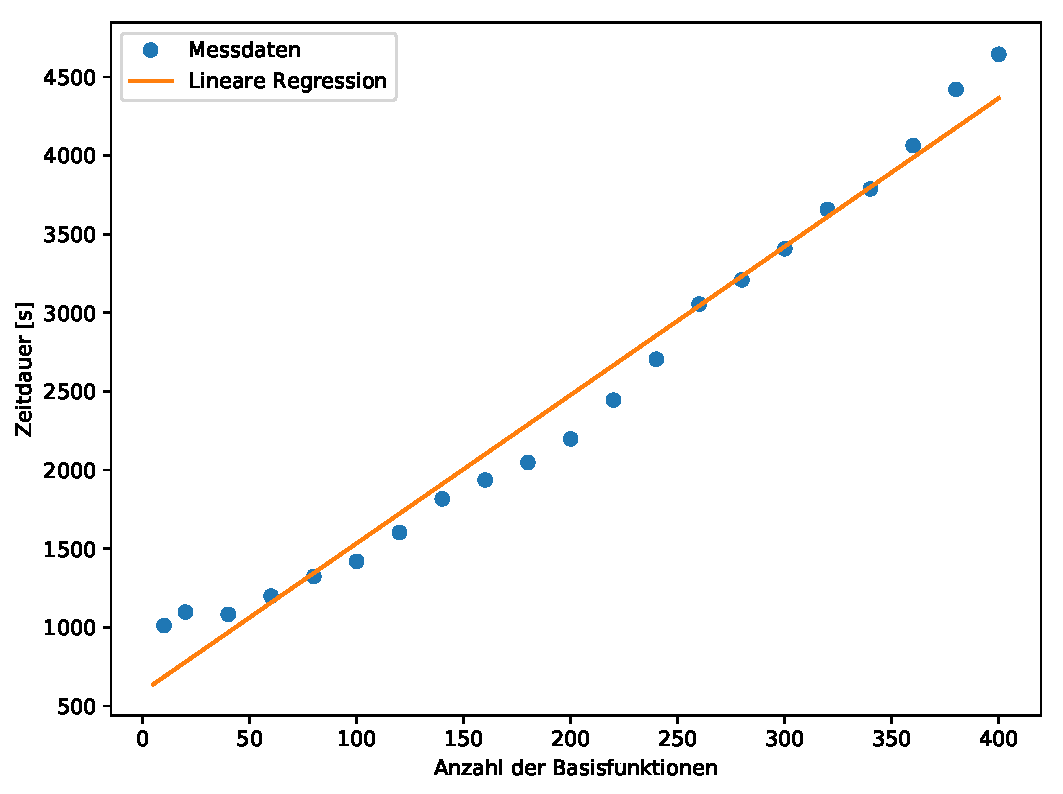
\includegraphics[width=4.2in]{figures/results/cross_prediction/rbf_placements_uv_time.pdf}
		\caption{Abhängigkeit der Laufzeit von $l$.}
	\end{subfigure}%
	\caption{Darstellung der Abhängigkeit des benötigten Laufzeit von der Anzahl der Basisfunktionen $l$ für das \textit{Barkley}-Modell\textit{Mitchell-Schaeffer}-Modell bei der Verwendung radialer Basisfunktionen.}
	\label{fig:exp_cross_rbf_placements_time_barkley}
\end{figure}

\begin{figure}[h]
	\centering
	\begin{subfigure}{\textwidth}
		\centering
		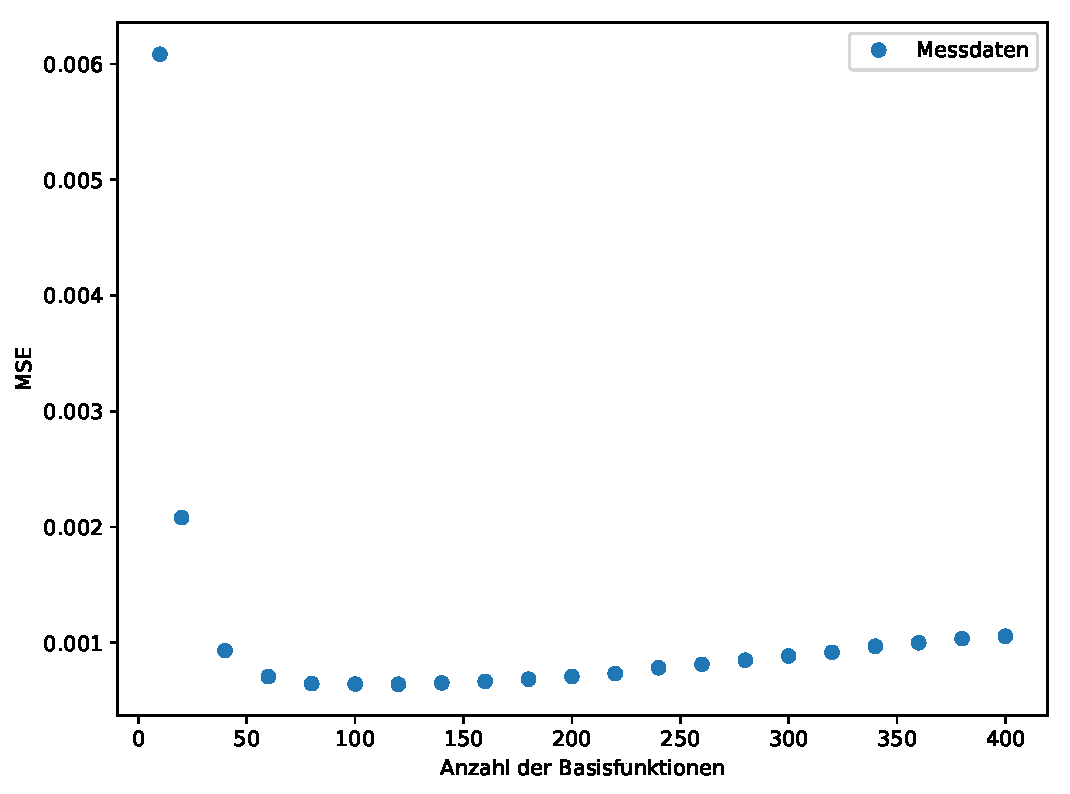
\includegraphics[width=4.2in]{figures/results/cross_prediction/rbf_placements_uv_mse.pdf}
  		\caption{Abhängigkeit des \textit{MSE}s von $l$.}
	\end{subfigure}%
	
	\caption{Darstellung der Abhängigkeit des MSE (unten) von der Anzahl der Basisfunktionen $l$ für das \textit{Barkley}-Modell\textit{Mitchell-Schaeffer}-Modell bei der Verwendung radialer Basisfunktionen.}
	\label{fig:exp_cross_rbf_placements_mse_barkley}
\end{figure}

Bei der Untersuchung des Zusammenhangs zwischen MSE und der Anzahl der Basisfunktionen kann zum einen ein asymptotischer Anteil erkannt werden, sodass der Fehler zuerst für mehr Basisfunktionen abnimmt. Allerdings lässt das Verhalten für das \textit{Mitchell-Schaeffer}-Modell erahnen, dass es hierbei einen optimalen Wert gibt, ab dem der Fehler wieder ansteigt. Dies kann durch eine schlechtere Generalisierung der Dynamik und ein zu starkes Anpassen und die Trainingsphase (auch bekannt als \textit{Overfitting}) erklärt werden. Zusammenfassend zeigt sich, dass die Wahl von $100$ Basisfunktionen eine akzeptable Abschätzung ist, sodass der Fehler möglichst gering ist und die Laufzeit auch gering gehalten wird. Diese Annahme wird im Folgenden ohne weitere qualitative Untersuchungen auf die anderen beiden Probleme übertragen, um den benötigten Rechenaufwand für die Parametersuche in einem angebrachten Rahmen zu halten.  

\FloatBarrier
\subsection{Echo State Network}
Abschließend ist dieses Problem nun mit den \textit{ESN}s gelöst worden. Dazu sind die Hyperparameter nach Abschnitt \ref{sec:exp_general_esn} gesucht worden. Die gefundenen Parameter und die damit erreichten Ergebnisse sind in Tabelle \ref{tab:exp_cross_esn_results} aufgelistet. Es ist auffällig, dass die optimalen Werte für $\sigma$ und $\Delta \sigma$ hier von denen der NN- und der RBF-Vorhersage abweichen. Auffällig ist, dass für beide Modelle die gleichen Hyperparameter die höchste Genauigkeit erzielen.\improvement{Add more details?} \\

\begin{table}[h]
	\centering
	\captionsetup{width=0.9\linewidth}
	\begin{tabular}{ccc}
		\hline		
		\multicolumn{1}{c}{} &  Barkley & Mitchell-Schaeffer \\ 
		\hline 
		\rule[-1ex]{0pt}{2.5ex} $\sigma$ & $3$ & $3$ \\ 
		\rule[-1ex]{0pt}{2.5ex} $\Delta \sigma$ & $1$ & $1$ \\ 
		\rule[-1ex]{0pt}{3.5ex} $N$ & $400$ & $400$ \\ 
		\rule[-1ex]{0pt}{3.5ex} $\rho(|\mathbf{W}|)$ & $0.95$ & $0.95$\\ 
		\rule[-1ex]{0pt}{3.5ex} $\alpha$ & $0.05$ & $0.05$ \\ 
		\rule[-1ex]{0pt}{3.5ex} $\epsilon$ & $0.1$ & $0.1$ \\ 
		\rule[-1ex]{0pt}{3.5ex} $\nu_{max}$ & $\num{1e-4}$ & $\num{1e-4}$\\ 
		\rule[-1ex]{0pt}{3.5ex} $\lambda$ & $\num{5e-6}$ & $\num{5e-6}$\\ 
		\rule[-1ex]{0pt}{2.5ex} Laufzeit [s] & $3710$ & $3733$ \\ 
		\rule[-1ex]{0pt}{2.5ex} \textbf{MSE} & \textbf{$\num{8.7e-7}$} & \textbf{0.00075} \\ 
		\rule[-1ex]{0pt}{2.5ex} \textbf{NRMSE} & \textbf{0.0039} & \textbf{0.1859} \\ 
		\hline 
	\end{tabular} 
	\caption{Ermittelte Hyperparameter des \textsc{ESN} für das \textit{Mitchell-Schaeffer}- und das \textit{Barkley}-Modell, welche zu den geringsten Fehlern führen.}
	\label{tab:exp_cross_esn_results}
\end{table}

Zuvor ist die Annahme getroffen worden, dass die Dynamik sich an jedem Punkt im Inneren des Feldes lokal ähnelt. Um diese Annahme zu untersuchen bietet es sich an die unterschiedlichen trainierten Gewichtsmatrizen $\mathbf{W_{out}}$ zu betrachten. Dies ist exemplarisch für die ermittelten Hyperparameter für das \textit{Barkley}-Modell durchgeführt und in Abbildung \ref{fig:exp_cross_esn_weights} dargestellt. Dabei gibt die vertikale Achse den Index $i$ des $i$-ten Eintrages von $\mathbf{W_{out}}$ an. Dafür sind die Matrizen $\mathbf{W_{out}} \in \mathbb{R}^{(1 + N_u + N) \times 1}$ mit $N_u = 9$ jeweils spaltenweise für $900$ Pixel in einem $30 \times 30$ Einheiten messendem Quadrat in der Mitte des Feldes aufgetragen.

\begin{figure}[H]
	\centering
	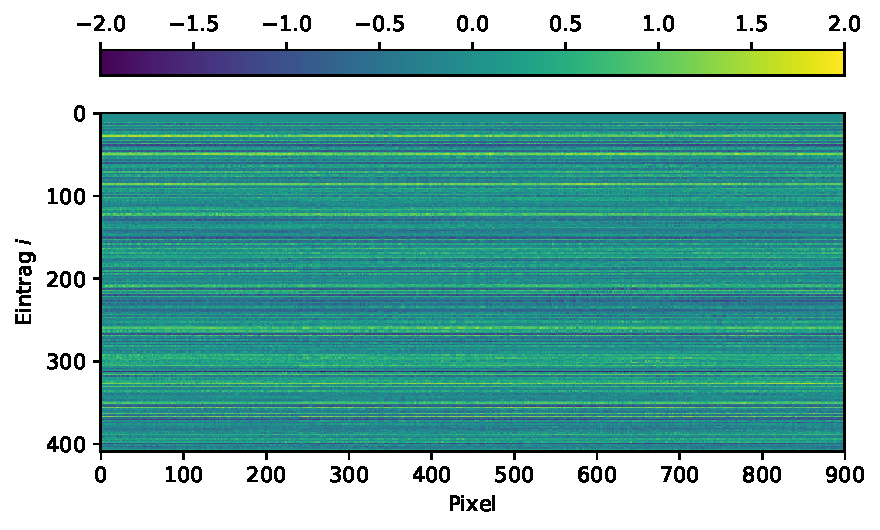
\includegraphics[height=3.0in]{figures/results/cross_prediction/weights.pdf}
	\setcapmargin[1cm]{1cm}
	\caption{Exemplarische Darstellung der Einträge der Gewichtsmatrix $\mathbf{W_{out}}$ des \textsc{ESN} für das \textit{Barkey}-Model anhand von $900$ verschiedene Bildpunkten, wobei$\mathbf{W_{out}}$ jeweils als Spalte in der Grafik dargestellt ist.}
	\label{fig:exp_cross_esn_weights}
\end{figure}

Dabei ist eine große Ähnlichkeit innerhalb der einzelnen Matrizen zu erkennen. So sind einige markante Linien in der Abbildung zu erkennen. So sind gewisse Einträge bei den Matrizen aller Pixel relativ stark beziehungsweise schwach. Trotzdem ist noch eine gewisse Varianz zuerkennen. Vermutlich wird sie dadurch verursacht, dass innerhalb der endlichen Trainingszeit nicht alle Dynamiken an jedem Pixel auftreten. Zusammenfassend kann dies als eine Bestätigung der Annahme der lokalen Ähnlichkeit gesehen werden. In weiteren Arbeiten bietet es sich an diese Frage weiter zu untersuchen und den Effekt dahingehend auszunutzen, als dass die Trainingsdaten mehrerer Punkte zusammengefasst werden können, sodass bereits aus einer kurzen Trainingszeit eine ausreichende Menge an Trainingsdaten gewonnen werden kann.
\improvement{Write something about the vanishing first 9 entries?}

\FloatBarrier
\subsection{Vergleich}
Abschließend kann nun ein Vergleich der drei verwendeten Methoden hinsichtlich ihrer Laufzeit und der erzielten Genauigkeiten durchgeführt werden. Dieser ist in Tabelle \ref{tab:exp_cross_comparison_results} zu finden. Die jeweils  besten Ergebnisse sind hervorgehoben. Die \textit{ESN}s erzielen für beide Modelle den geringsten Fehler, also die höchste Genauigkeit. Dabei ist der NRMSE für das \textit{Barkley}-Modell mehrere Größenordnung kleiner als bei den Konkurrenz-Ansätzen. Diese überaus hohe Genauigkeit ist für das \textit{Mitchell-Schaeffer}-Modell nicht erreicht worden. Hier beträgt der Fehler trotzdem etwa nur ein Drittel von dem der anderen Ansätze. Im Austausch für diese hohe Genauigkeit ist allerdings die benötigte Zeit für die Vorhersage höher als bei den Konkurrenten. Unter der Voraussetzung, dass die Rechenzeit nur eine untergeordnete Rolle spielt, so ergeben sich die \textit{ESN}s als bester Ansätze für die Kreuz-Prädiktion.
\begin{table}[h]
	\centering
	\captionsetup{width=0.9\linewidth}
	\begin{tabular}{cccccccc}
		\hline		
		\multicolumn{1}{c}{} & \multicolumn{3}{c}{Barkley} & \multicolumn{3}{c}{Mitchell-Schaeffer}		\\
		%\cline{2-7}
		\multicolumn{1}{c}{} & NN & RBF & ESN & NN & RBF & ESN \\
		
		\hline
		
		Laufzeit [s] 	& \textbf{40} 		& 1430		& 3710		& 5252		& \textbf{1434} 		& 3733 \\
		MSE 			& 0.00098	& 0.01046	& \textbf{\num{8.7e-7}} 	& 0.01891	& 0.00948 	& \textbf{0.00075} \\
		NRMSE 			& 0.1317	& 0.1023	& \textbf{\num{0.0039}} 	& 0.8795	& 0.6228 	& \textbf{0.1859} \\
		\hline 
	\end{tabular} 
	\caption{Vergleich der benötigten Laufzeit und der erreichten Fehlers der drei Ansätze für das \textit{Mitchell-Schaeffer}- und das \textit{Barkley}-Modell, welche zu den geringsten Fehlern führen.}
	\label{tab:exp_cross_comparison_results}
\end{table}

\FloatBarrier
\section{Kreuz-Prädiktion innere Dynamiken}
\label{sec:exp_inner_prediction}
Bei Messungen der elektrischen Erregung des Herzens können nach aktuellen Stand meistens nur die Erregungen auf der Herzoberfläche gemessen werden. Die Ausbreitungen im Inneren des räumlich ausgedehnten Herzens bleiben somit verborgen. Zudem ist anzunehmen, dass die Gesamtdynamik nicht nur durch die Oberfläche, sondern auch durch die Erregung im Inneren bestimmt und charakterisiert wird. Somit wird die Frage aufgeworfen, ob die innere Erregung des Herzens nur durch die Kenntnis der Oberflächendynamik vorhergesagt werden kann. In diesem Abschnitt soll versucht werden, diese Fragestellung erneut mit den \textsc{ESN}s und den klassischen Methoden zu untersuchen. Dabei wird diese Frage statt an einem dreidimensionalen Systems an den zuvor bereits benutzten zweidimensionalen Modellen untersucht.\\

\begin{figure}[h]
	\centering
	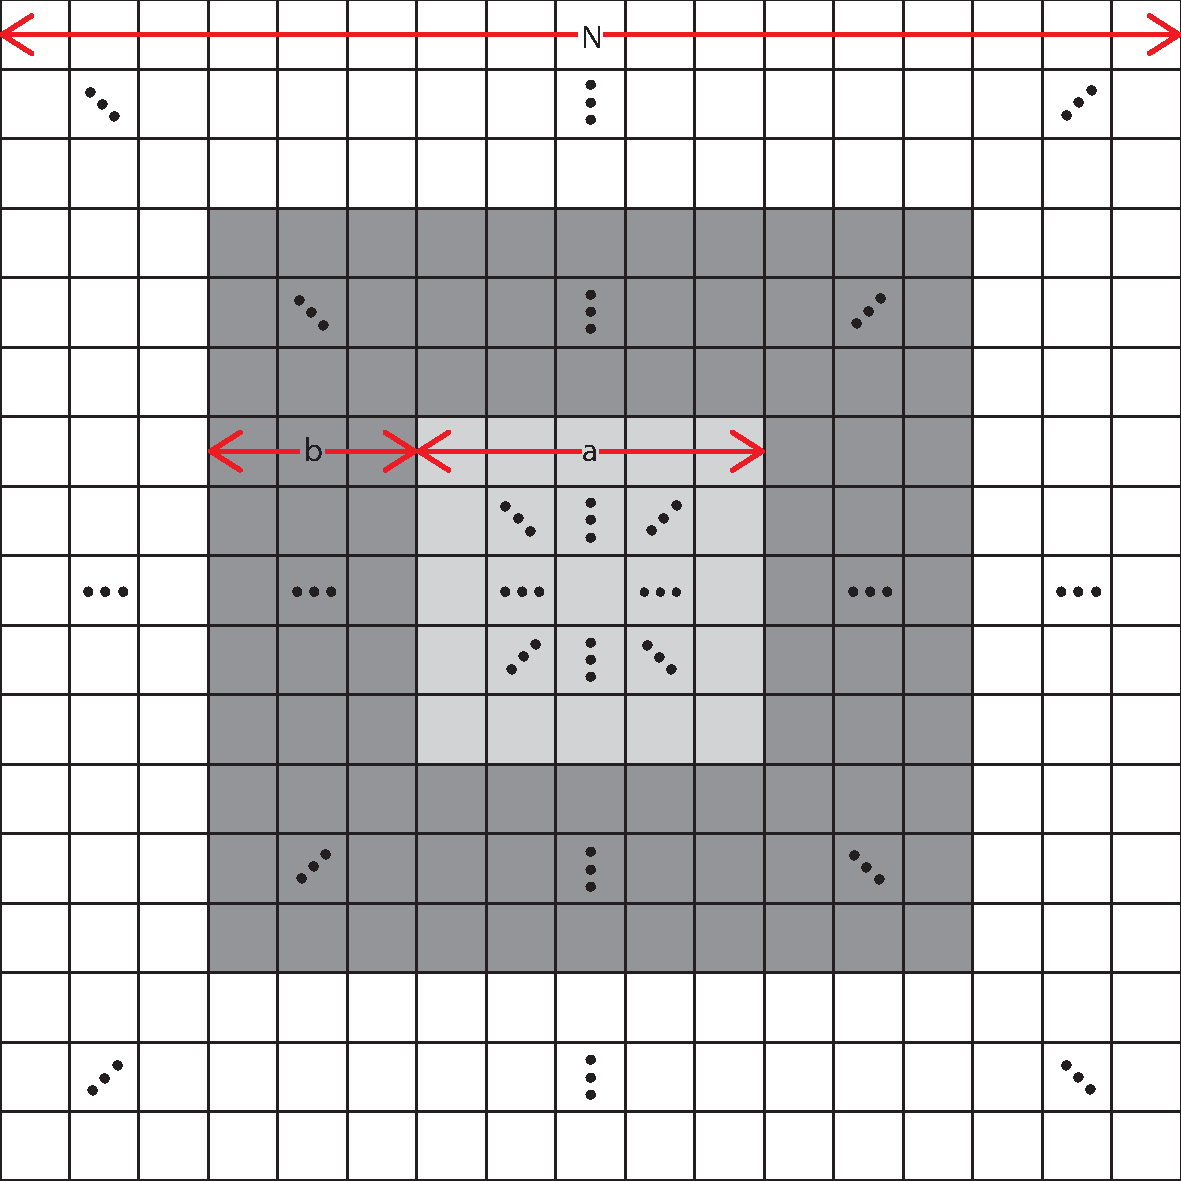
\includegraphics[width=.4\linewidth]{figures/illustrations/inner_prediction.pdf}
	\caption{Darstellung des Aufbaus. Das gesamte $N \times N$ große Feld der Spannungsvariable ist in weiß, wohingegen der vorherzusagende Bereich der Größe $a \times a$ in hellgrau dargestellt ist. Drumherum liegt der dunkelgraue Rahmen der Größe $b \times b$ dessen Pixel für die Vorhersage des Inneren genutzt werden.}
	\label{fig:exp_inner_prediction}
\end{figure}

Hierbei wird nur das Feld der Spannungsvariable betrachtet. In diesem $N \times N$ Einheiten großem Feld wird ein Quadrat mit der Seitenlänge $a$ ausgewählt, für dessen Pixel die Spannungsvariable bestimmt werden soll. Dazu wird um das innere Quadrat ein Rahmen der Breite $b$ gewählt und die Spannungsvariable der beinhalteten Pixel als Quelle genutzt. Eine graphische Illustration dieses Aufbaus ist in Abbildung \ref{fig:exp_inner_prediction} dargestellt. Somit wird die Spannung im Inneren für $a^2$ Punkte durch die Kenntnis der $(a+2b)^2-a^2$ umgebenden Pixel bestimmt.\\

Dieses Szenario ist für die in Tabelle \ref{tab:exp_inner_cross_pred_parameter} angegebenen Parameterkombinationen durchgeführt worden. Im Folgenden werden jeweils nur die gefundenen Hyperparameter und Ergebnisse für den $b$ Wert vorgestellt, der zu dem geringsten Fehler führt.

\begin{table}[h]
	\centering
	\begin{tabular}{cccc|ccc|ccc|ccc|ccc|ccc|cc|c}
		\hline
		$a$ & \multicolumn{3}{c|}{4} & \multicolumn{3}{c|}{8} & \multicolumn{3}{c|}{16} & \multicolumn{3}{c|}{32} & \multicolumn{3}{c|}{64} & \multicolumn{3}{c|}{128*} & \multicolumn{2}{c|}{146*} & 148* \\
		\hline
		$b$ & 1 & 2 & 3 & 1 & 2 & 3 & 1 & 2 & 3 & 1 & 2 & 3 & 1 & 2 & 3 & 1 & 2 & 3 & 2 & 1 & 1 \\
		\hline
	\end{tabular} 
	\caption{Verwendete Parameter $a$ und $b$ für die Abmessungen des inneren und äußeren Quadrates. Die markierten Werte sind nur für die \textsc{ESN}s untersucht worden.}
	\label{tab:exp_inner_cross_pred_parameter}
\end{table} 

\subsection{Nächste Nachbar Vorhersage}
Für die letzte Aufgabe ist erneut zuerst der \textsc{NN}-Ansatz getestet worden. Es ist anzumerken, dass dies nicht alle Parameterkombinationen $a$, $b$ aus Tabelle \ref{tab:exp_inner_cross_pred_parameter} durchgeführt worden ist, da der Rechenaufwand teilweise zu groß geworden ist. Dies liegt daran, dass die Dimension der Eingabevariablen mit
\begin{align*}
(a+2b)^2-a^2 = 4b^2+4ab
\end{align*}
skaliert. Da zudem die Rechenzeit für diesen Ansatz nach \ref{sc:theory_nn} für wachsende Dimensionen sehr stark zunimmt, kann diese Aufgabe für große Abmessungen des vorherzusagendenen Bereiches nicht mehr in einer angebrachten Zeit berechnet werden.
Die optimalen gefundenen Hyperparameter und die damit erreichten Ergebnisse sind in Tabelle \ref{tab:exp_inner_cross_nn_results} aufgelistet.

\begin{table}[h]
	\centering

	\begin{tabular}{ccccccccccc}
		\hline		
		\multicolumn{1}{c}{} & \multicolumn{5}{c}{Barkley}\\ 
		\hline 
		\rule[-1ex]{0pt}{2.5ex} $a$ & 4 & 8 & 16 & 32 & 64\\ 
		\rule[-1ex]{0pt}{2.5ex} $b$ & 1 & 1 & 1  & 1  & 1 \\ 
		\rule[-1ex]{0pt}{2.5ex} $\delta$ & 4 & 4 & 4 & 3 & 3 \\ 
		\rule[-1ex]{0pt}{2.5ex} k & 5 & 5 & 5 & 5 & 5 \\ 
		\rule[-1ex]{0pt}{2.5ex} Laufzeit [s] & $\approx 1$ & 8 & 287 & 1809 & 14754\\ 
		\rule[-1ex]{0pt}{2.5ex} \textbf{MSE} & \textbf{0.00231} & \textbf{0.00891} & \textbf{0.07097} & \textbf{0.18961} & \textbf{0.24599}\\ 
		\rule[-1ex]{0pt}{2.5ex} \textbf{NRMSE} & \textbf{0.0155} & \textbf{0.0596} & \textbf{0.4779} & \textbf{1.3032} & \textbf{1.7009} \\ 
		\hline 
	\end{tabular} 
	
	\vspace{0.75cm}

	\centering

	\begin{tabular}{ccccccccccc}
		\hline
		\multicolumn{1}{c}{} & \multicolumn{5}{c}{Mitchell-Schaeffer} \\ 
		\hline 
		\rule[-1ex]{0pt}{2.5ex} $a$ & 4 & 8 & 16 & 32 & 64 \\ 
		\rule[-1ex]{0pt}{2.5ex} $b$ & 1 & 1 & 1  & 1  & 1\\ 
		\rule[-1ex]{0pt}{2.5ex} $\delta$ & 3 & 3 & 3 & 4 & 4 \\ 
		\rule[-1ex]{0pt}{2.5ex} k & 5 & 5 & 5 & 5 & 5 \\ 
		\rule[-1ex]{0pt}{2.5ex} Laufzeit [s] & $\approx 1$ & 17 & 194 & 2482 & 20272\\ 
		\rule[-1ex]{0pt}{2.5ex} \textbf{MSE} & \textbf{0.14221} & \textbf{0.02465} & \textbf{0.06460} & \textbf{0.08744} & \textbf{0.09283} \\ 
		\rule[-1ex]{0pt}{2.5ex} \textbf{NRMSE} & \textbf{0.2663} & \textbf{0.4052} & \textbf{0.9779} & \textbf{1.3564} & \textbf{1.4012} \\ 
		\hline 
	\end{tabular} 

	\caption{Ermittelte Hyperparameter der nächsten Nachbar Vorhersage und Werte für $b$ für das \textit{Barkley}-Modell (oben) und das \textit{Mitschell-Schaeffer}-Modell (unten) für verschiedene Größen $a$ des vorherzusagenden Bereichs, welche zu den geringsten Fehlern führen.}
\label{tab:exp_inner_cross_nn_results}
\end{table}

Dabei ist zu erkennen, dass die Qualität der Vorhersage mit steigendem $a$ stark abnimmt. So kann für das \textit{Barkley}-Modell nur für $a \in \{4,8\}$ ein NRMSE der deutlich unter $0.50$ erreicht werden. Für größere Bereiche steigt der NRMSE sogar auf $> 1.0$ an, sodass die Vorhersage nicht mehr genauer ist als eine naive Vorhersage mittels des Mittelwertes des Trainingsdatensatzes. Die Vorhersagen des \textit{Mitchell-Schaeffer}-Modells zeigen eine gleichartige Tendenz, doch ist hier der Fehler für die kleinste innere Abmessung $a=4$ deutlich stärker als im \textit{Barkley}-Modell.

\FloatBarrier
\subsection{Radiale Basisfunktionen}
Analog zu den vorherigen Ausführungen sind die radialen Basisfunktionen ebenfalls auf dieses Problem angewendet worden. Dabei ist mit einer analogen Begründung wie bei den nächsten Nachbarn nur der eingeschränkte Wertebereich für $a$ durchlaufen worden. Die dafür gefundenen Hyperparameter und die Fehler können in Tabelle \ref{tab:exp_inner_cross_rbf_results} gefunden werden.
\begin{table}[h]
	\centering

	\begin{tabular}{ccccccccccc}
		\hline
		\multicolumn{1}{c}{} & \multicolumn{5}{c}{Barkley}\\ 
		\hline
		\rule[-1ex]{0pt}{2.5ex} $a$ & 4 & 8 & 16 & 32 & 64\\ 
		\rule[-1ex]{0pt}{2.5ex} $b$ & 1 & 1 & 1  & 1  & 1 \\ 
		\rule[-1ex]{0pt}{2.5ex} $\delta$ & 4 & 4 & 4 & 3 & 3 \\ 
		\rule[-1ex]{0pt}{2.5ex} $\sigma_{RBF}$ & 9 & 5 & 9 & 9 & 7\\ 
		\rule[-1ex]{0pt}{2.5ex} Laufzeit [s] & $\approx 2$ & 7 & 41 & 279 & 1845\\ 
		\rule[-1ex]{0pt}{2.5ex} \textbf{MSE} & \textbf{0.00051} & \textbf{0.00450} & \textbf{0.04009} & \textbf{0.08783} & \textbf{0.13615}\\ 
		\rule[-1ex]{0pt}{2.5ex} \textbf{NRMSE} & \textbf{0.0586} & \textbf{0.1735} & \textbf{0.5196} & \textbf{0.7769} & \textbf{0.9703} \\ 
		\hline 
	\end{tabular} 
	
	\vspace{0.75cm}

	\centering

	\begin{tabular}{ccccccccccc}
		\hline
		\multicolumn{1}{c}{} & \multicolumn{5}{c}{Mitchell-Schaeffer} \\ 
		\hline 
		\rule[-1ex]{0pt}{2.5ex} $a$ & 4 & 8 & 16 & 32 & 64 \\ 
		\rule[-1ex]{0pt}{2.5ex} $b$ & 1 & 1 & 1  & 1  & 1\\ 
		\rule[-1ex]{0pt}{2.5ex} $\delta$ & 3 & 3 & 3 & 4 & 4 \\ 
		\rule[-1ex]{0pt}{2.5ex} $\sigma_{RBF}$ & 9 & 9 & 9 & 5 & 7 \\ 
		\rule[-1ex]{0pt}{2.5ex} Laufzeit [s] & $\approx 1$ & 7 & 43 & 237 & 1756\\
		\rule[-1ex]{0pt}{2.5ex} \textbf{MSE} & \textbf{0.00064} & \textbf{0.00497} & \textbf{0.02220} & \textbf{0.04745} & \textbf{0.05588} \\ 
		\rule[-1ex]{0pt}{2.5ex} \textbf{NRMSE} & \textbf{0.1094} & \textbf{0.2857} & \textbf{0.5797} & \textbf{0.8580} & \textbf{0.9184} \\ 
		\hline 
	\end{tabular} 

	\caption{Ermittelte Hyperparameter der radialen Basisfunktionen und Werte für $b$ für das \textit{Barkley}-Modell (oben) und das \textit{Mitchell-Schaeffer}-Modell (unten) für verschiedene Größen $a$ des vorherzusagenden Bereichs, welche zu den geringsten Fehlern führen.}
\label{tab:exp_inner_cross_rbf_results}
\end{table}

Es ist anzumerken, dass der NRMSE für beide Modelle und alle betrachteten Größen $a$ kleiner als $1.0$ bleibt. Nichtsdestotrotz steigt er ebenfalls mit wachsendem $a$ an, wie schon bei den nächsten Nachbarn. Für die größten beiden $a$-Werte ist in beiden Modellen der Fehler allerdings schon so groß, dass die Vorhersage kaum nützliche Informationen liefert.

\FloatBarrier
\subsection{Echo State Network}
Im Gegensatz zu den anderen beiden Methoden wächst die benötigte Rechenzeit bei der Verwendung der \textsc{ESN}s nicht so schnell an, sodass hiermit auch deutlich größere innere Felder betrachtet werden können. Zur Optimierung des Ansatzes ist erneut das in Abschnitt \ref{sec:exp_general_esn} beschriebene Verfahren durchgeführt worden. Es ist allerdings so modifiziert worden, dass bei der groben Hyperparameterbestimmung des \textsc{ESN} nicht vier statt einem Punkt des inneren Quadrates betrachtet worden sind.\\

Zudem ergibt sich bei dieser Aufgabe ein weiteres Problem, welches eine Modifikation erfordert: In den vorherigen Aufgaben ist die Dimension des Eingangssignals in das \textsc{ESN} $N_u < 50$ gewesen. Nun wächst die Dimension des Eingangssignals allerdings sehr stark mit $N_u = 4b(b+a)$ an. Dies würde bei der Konstruktion der Eingangsmatrix $\mathbf{W_{in}}$ nach Abschnitt \ref{sec:esn_structure} dazu führen, dass die inneren Einheiten des Reservoirs zu viele Eingangssignale erhalten und somit unter Umständen schnell eine Sättigung des $tanh(\cdot)$ in der zeitlichen Entwicklungsgleichung \ref{eq:esn_stateeq} ergibt. Um dies zu lösen ist ein neuer Hyperparameter $\eta$ eingeführt worden, der die Anzahl von Eingangssignalen pro innerer Einheit beschränkt. Dadurch wird die Matrix $\mathbf{W_{in}}$ dünn besetzt. Dies wird zudem dadurch motiviert, dass viele Einträge des Eingangssignals aus Bildpunkten mit einem geringen Abstand zueinander stammen, wodurch redundante Informationen eingespeist werden würden. Durch eine dünn besetzte Matrix $\mathbf{W_{in}}$ kann dieser Effekt reduziert werden. Des Weiteren wird versucht eine reichhaltigere innere Dynamik durch diesen Schritt analog zu der Begründung der Dünnbesetztheit der Matrix $\mathbf{W}$ zu erzeugen.\\

Bei der Untersuchung ist zusätzlich ersichtlich geworden, dass der untersuchte Bereich der Regularisierung $\lambda \in [\num{5e-2},\num{5e-6}]$ zu gering ist, da der optimale Wert stets am linken Rand des Intervalls gefunden worden ist. Deswegen ist zusätzlich einmal eine Suche auf dem größeren Parameterbereich $\lambda \in [\num{5e-4},\num{5e+4}]$ durchgeführt worden.
In Tabelle \ref{tab:exp_inner_cross_esn_results} sind die Fehler und benötigten Laufzeiten für die besten Reservoirs für die beiden Modelle aufgelistet. Es kann erneut der Trend beobachtet werden, dass der Fehler mit steigendem $a$ ebenso zunimmt, und für kleine Werte für $a$ der Fehler im \textit{Mitchell-Schaffer}-Modell größer ist als im \textit{Barkley-Modell}.

\begin{table}[h]
	\centering

	\resizebox{\columnwidth}{!}{%
		\begin{tabular}{cccccccc}
			\hline
			\multicolumn{1}{c}{} & \multicolumn{7}{c}{Barkley}\\ 
			\hline 
			\rule[-1ex]{0pt}{2.5ex} $a$ & 4 & 8 & 16 & 32 & 64 & 128 & 148\\ 
			\rule[-1ex]{0pt}{2.5ex} $b$ & 1 & 1 & 1 & 1 & 1 & 1 & 1 \\ 
			\rule[-1ex]{0pt}{2.5ex} Laufzeit [s] & 5 & 15 & 60 & 170 & 1922 & 3320 & 2970\\
			\rule[-1ex]{0pt}{2.5ex} \textbf{MSE} & \textbf{0.00005} & \textbf{0.00111} & \textbf{0.01447} & \textbf{0.09301} & \textbf{0.13093} & \textbf{0.15106} & \textbf{0.18380}\\ 
			\rule[-1ex]{0pt}{2.5ex} \textbf{NRMSE} & \textbf{0.0121} & \textbf{0.0801} & \textbf{0.3386} & \textbf{0.7398} & \textbf{0.9438} & \textbf{1.0098} & \textbf{1.1049} \\ 
			\hline 
		\end{tabular} 
	}
	
	\vspace{0.75cm}

	\centering

	\resizebox{\columnwidth}{!}{%
		\begin{tabular}{cccccccc}
			\hline
			\multicolumn{1}{c}{} & \multicolumn{7}{c}{Mitchell-Schaeffer}\\ 
			\hline
			\rule[-1ex]{0pt}{2.5ex} $a$ & 4 & 8 & 16 & 32 & 64 & 128 & 148\\ 
			\rule[-1ex]{0pt}{2.5ex} $b$ & 1 & 1 & 1 & 1 & 1 & 1 & 1 \\ 
			\rule[-1ex]{0pt}{2.5ex} Laufzeit [s] & 3 & 9 & 27 & 121 & 548 & 3322 & 3021\\
			\rule[-1ex]{0pt}{2.5ex} \textbf{MSE} & \textbf{0.00023} & \textbf{0.00177} & \textbf{0.02969} & \textbf{0.05061} & \textbf{0.06330} & \textbf{0.06842} & \textbf{0.06761}\\ 
			\rule[-1ex]{0pt}{2.5ex} \textbf{NRMSE} & \textbf{0.0661} & \textbf{0.1704} & \textbf{0.6703} & \textbf{0.8861} & \textbf{0.9775} & \textbf{1.0166} & \textbf{1.0049} \\ 
			\hline 
		\end{tabular} 
	}

	\caption{Ermittelte Hyperparameter der \textsc{ESN}s und Werte für $b$ für das \textit{Barkley}-Modell (oben) und das \textit{Mitchell-Schaeffer}-Modell (unten) für verschiedene Größen $a$ des vorherzusagenden Bereichs, welche zu den geringsten Fehlern führen.}
\label{tab:exp_inner_cross_esn_results}
\end{table}

Es ist anzunehmen, dass für die Vorhersage eines Punktes der weit von den bekannten Randwerten entfernt liegt, nicht nur durch sein vorheriger Wert und die aktuellen Randwerte benötigt werden. Vielmehr werden die vergangenen Randwerte einen starken Einfluss nehmen. Dies kann an einem Beispiel schnell deutlich gemacht werden: Würde beispielsweise eine ebene Welle durch das Feld propagieren, so können weit entfernte Punkte erst deutlich nachdem die Welle durch die Ränder hindurch gelaufen ist, hiervon beeinflusst werden. Somit benötigt das System eine ausgeprägte Gedächtnisleistung. Bei den \textsc{ESN}s skaliert nach \ref{sc:esn} die Gedächtnisleistung mit der Größe $N$ des Netzwerkes. Es wäre also anzunehmen, dass möglichst große Reservoirs eine optimale Leistung erzielen können. Dies kann experimentell nicht bestätigt werden. So erzielen zwar teilweise die größtmöglichen Reservoirs ($N=400$) die besten Ergebnisse, doch tritt gibt es auch Werte für $a$ bei denen kleinere Reservoirs ($N=50$) besser arbeiten.\\

\begin{figure}[h]
	\centering
	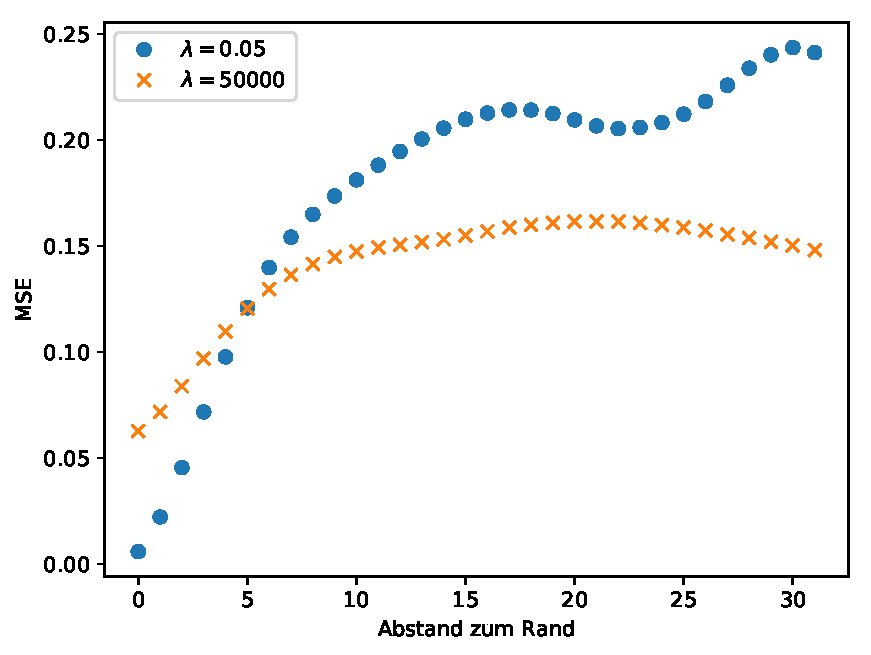
\includegraphics[height=2.5in]{figures/results/inner_cross_prediction/inner_errors.pdf}
	\setcapmargin[1cm]{0.5cm}
	\caption{Graphische Darstellung der Abhängigkeit des MSE für die Vorhersage der $u$-Variable des \textit{Barkley}-Modells vom Abstand zum Rand. In blau ist die Abhängigkeit für das \textsc{ESN}s mit starker und in orange für das mit schwacher Regularisierung dargestellt.}
	\label{fig:exp_inner_cross_barkley_esn_error_dependency_comparison}
\end{figure} 

Um den Einfluss der Regularisierung hervorzuheben sind in Abbildung \ref{fig:exp_inner_cross_barkley_esn_comparison} die Vorhersagen des optimalen Reservoir mit der hohen Regularisierung ($\lambda=\num{5e4}$) und eines zuvor ermittelten Reservoirs mit einer geringeren Regularisierung ($\lambda=0.05$) exemplarisch für das \textit{Barkley}-Modell dargestellt. Es ist zu erkennen, dass im Falle der starken Regularisierung die Vorhersage stark verschwommen ist und beinahe der Mittelwert der Erregung anstelle der feineren Strukturen vorhergesagt wird. Dagegen wird bei der geringeren Regularisierung eine feinere Struktur vorhergesagt. \improvement{Add details?}
Zudem ist in Abbildung \ref{fig:exp_inner_cross_barkley_esn_error_dependency_comparison} die Abhängigkeit des mittleren quadratischen Fehlers für jene beiden Reservoirs dargestellt. Dabei ist zu erkennen, dass im für geringe Abstände die feine Vorhersage mit der kleinen Regularisierung deutlich geringere Fehler verursacht, wohingegen ab einem Abstand von $5$ Gitterpunkten eine stärkere Regularisierung geringere Fehler erzeugt. Zudem scheint der Fehler dabei schnell gegen eine obere Schranke zu konvergieren. Dies lässt sich damit vereinbaren, dass dieses Reservoir hauptsächlich noch den Mittelwert der Dynamik vorhersagt.

\begin{figure}[h]
	\centering
	\begin{subfigure}{.5\textwidth}
		\centering
		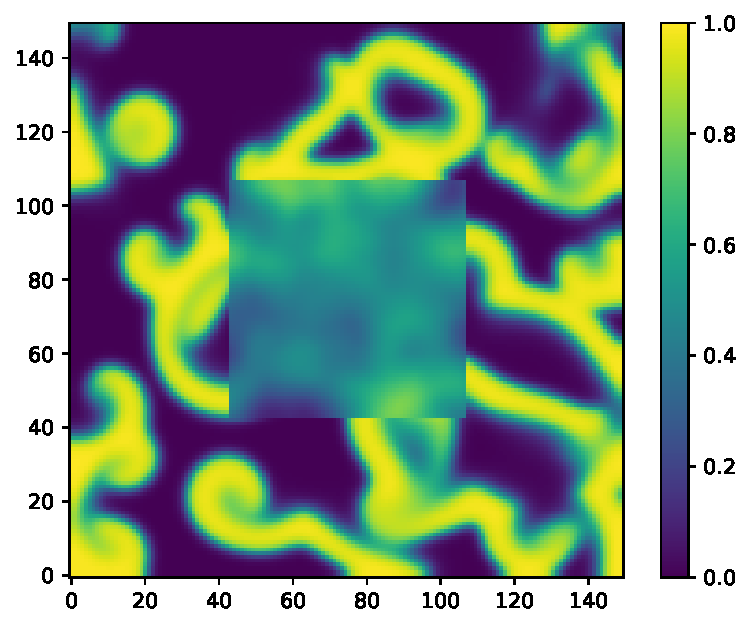
\includegraphics[height=2.5in]{figures/results/inner_cross_prediction/barkley_u_inner_esn_high_penalty.pdf}
		\setcapmargin[1cm]{0.5cm}
		\caption{Vorhersage des \textsc{ESN}s mit $\lambda=50000$}
	\end{subfigure}%
	\begin{subfigure}{.5\textwidth}
		\centering
		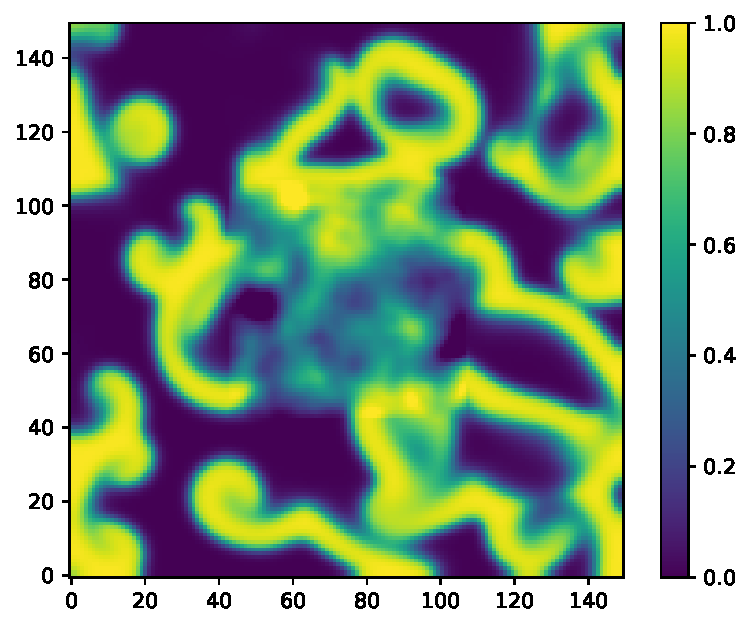
\includegraphics[height=2.5in]{figures/results/inner_cross_prediction/barkley_u_inner_esn_low_penalty.pdf}
		\setcapmargin[1cm]{0.5cm}
  		\caption{Vorhersage des \textsc{ESN}s mit $\lambda=0.05$}
	\end{subfigure}
	\caption{Graphische Darstellung der $u$-Variable des \textit{Barkley}-Modells für den $1000$. Zeitschritt des Evaluationsdatensatzes. Links ist die Vorhersagen des \textsc{ESN}s mit starker und rechts mit schwacher Regularisierung dargestellt.}
	\label{fig:exp_inner_cross_barkley_esn_comparison}
\end{figure} 

\subsection{Vergleich}
Für einen Vergleich der drei Methoden bietet es sich an die Ergebnisse für die größten Wert für $a$ durchzuführen, der mit allen drei Ansätzen betrachtet worden ist. Dies entspricht dem Wert $a=64$. Eine Übersicht der verschiedenen Ergebnisse ist in Tabelle \ref{tab:exp_inner_cross_comparison_results} zu finden.

\begin{table}[h]
	\centering
	\captionsetup{width=0.9\linewidth}
	\begin{tabular}{cccccccc}
		\hline
		\multicolumn{1}{c}{} & \multicolumn{3}{c}{Barkley} & \multicolumn{3}{c}{Mitchell-Schaeffer}		\\
		%\cline{2-7}
		\multicolumn{1}{c}{} & NN & RBF & ESN & NN & RBF & ESN \\
		
		\hline
		
		Laufzeit [s] 	& 20272 	& 1756		& \textbf{1089}		& 14754		&  	1845	& \textbf{1206} \\
		MSE 			& 0.09284	& 0.05588	& 	\textbf{0.05389} 		& 0.24599	& 0.13615 	& \textbf{0.12975}	 \\
		NRMSE 			& 1.1837	& 0.9184	& \textbf{0.9019} 			& 1.3042	& 0.9703 	& \textbf{0.9472} \\
		\hline 
	\end{tabular} 
	\caption{Vergleich der benötigten Laufzeit und der erreichten Fehlers der drei Ansätze für das \textit{Mitchell-Schaeffer}- und das \textit{Barkley}-Modell, welche zu den geringsten Fehlern führen, für $a=64$.}
	\label{tab:exp_inner_cross_comparison_results}
\end{table}

Es zeigt sich erneut, dass die Vorhersagen der klassischen Methoden einen höheren Fehler haben. Während der \textsc{NN}-Ansatz bei beiden Modellen schlechtere Ergebnisse als die Vorhersage mittels des Mittelwertes liefert, sind die radialen Basisfunktionen und die \textsc{ESN}s leicht besser als diese. Dabei erreichen die \textsc{ESN}s und radialen Basisfunktionen in etwa die gleiche Genauigkeit. Diese reicht allerdings auch nicht aus, um dies Methoden tatsächlich sinnvoll verwenden zu können. 

Des Weiteren wächst der Fehlers mit steigender Größe des vorherzusagenden Bereiches auch bei allen drei Ansätze an. Es ist somit zu vermuten, dass dies nicht nur eine reine Beschränkung der einzelnen Methoden ist, sondern dass es womöglich eine Eigenschaft der betrachteten Modelle ist. 
\improvement{Add comparison images}

\begin{figure}[h]
	\centering
	\begin{subfigure}{.5\textwidth}
		\centering
		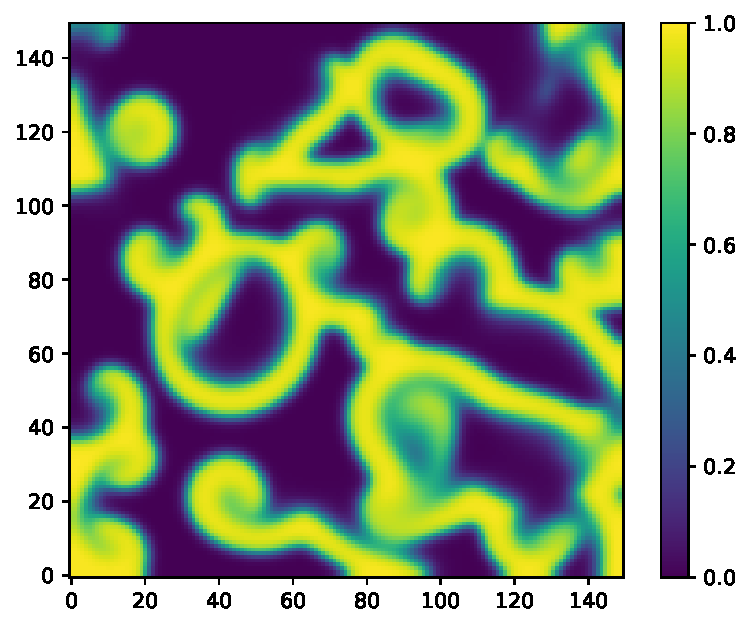
\includegraphics[height=2.5in]{figures/results/inner_cross_prediction/barkley_u_inner_original.pdf}
		\setcapmargin[1cm]{0.5cm}
		\caption{Echte Erregung des Modells}
		\label{fig:exp_inner_cross_barkley_result_orig}
	\end{subfigure}%
	\begin{subfigure}{.5\textwidth}
		\centering
		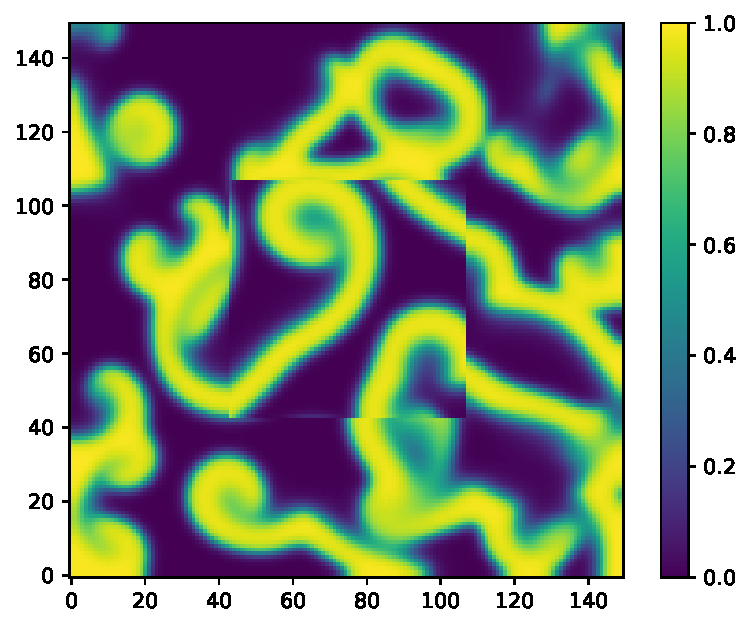
\includegraphics[height=2.5in]{figures/results/inner_cross_prediction/barkley_u_inner_nn.pdf}
		\setcapmargin[1cm]{0.5cm}
  		\caption{Vorhersage des \textsc{NN}-Ansatzes}
  		\label{fig:exp_inner_cross_barkley_result_nn_pred}
	\end{subfigure}
	\begin{subfigure}{.5\textwidth}
		\centering
		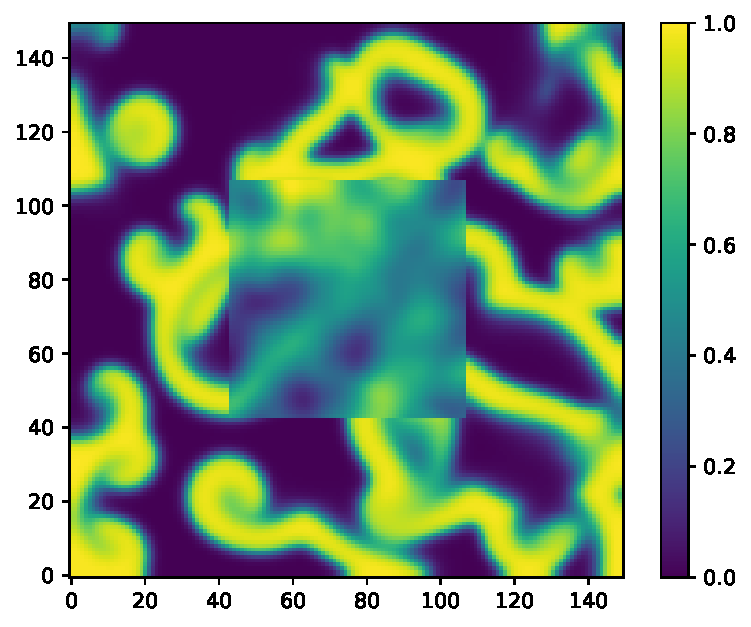
\includegraphics[height=2.5in]{figures/results/inner_cross_prediction/barkley_u_inner_rbf.pdf}
		\setcapmargin[1cm]{0.5cm}
  		\caption{Vorhersage des \textsc{RBF}-Ansatzes}
  		\label{fig:exp_inner_cross_barkley_result_rbf_pred}
	\end{subfigure}%
	\begin{subfigure}{.5\textwidth}
		\centering
		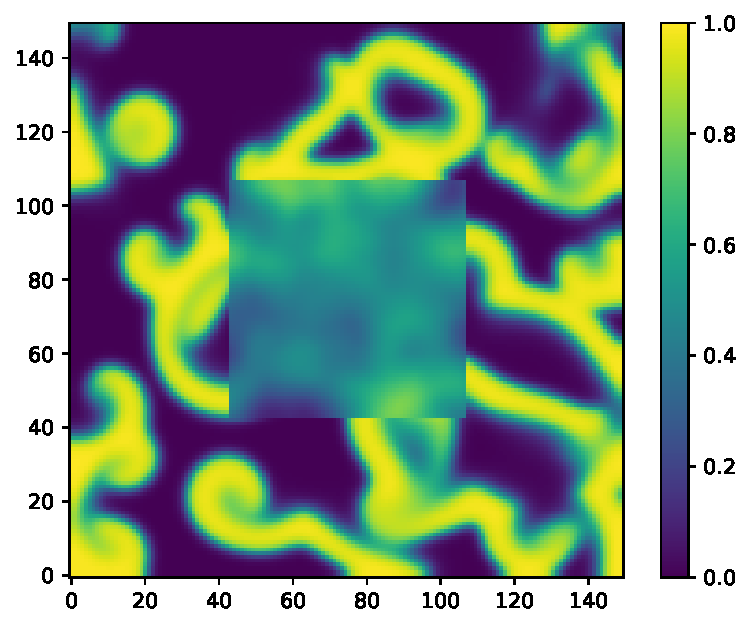
\includegraphics[height=2.5in]{figures/results/inner_cross_prediction/barkley_u_inner_esn.pdf}
		\setcapmargin[1cm]{0.5cm}
  		\caption{Vorhersage des \textsc{ESN}}
  		\label{fig:exp_inner_cross_barkley_result_esn_pred}
	\end{subfigure}
	\caption{Graphische Darstellung der $u$-Variable des \textit{Barkley}-Modells für den $1000$. Zeitschritt des Evaluationsdatensatzes für $a=64$. Oben links ist das tatsächliche Feld des Modells zu sehen. Danach folgenden im Uhrzeigersinn die Vorhersagen des \textsc{NN}-Ansatzes, des \textsc{RBF}-Ansatzes und des \textsc{ESN}.}
	\label{fig:exp_inner_cross_barkley_result}
\end{figure} 

In Abbildung \ref{fig:exp_inner_cross_barkley_result} werden exemplarisch die aus den drei Ansätzen resultierenden Felder der Spannungsvariable $u(t)$ des \textit{Barkley}-Modells zusammen mit dem originalen Feld dargestellt. Eine analoge Darstellung für das \textit{Mitchell-Schaeffer}-Modell ist im Anhang als Abbildung \ref{fig:apx_inner_cross_mitchell_result} zu finden. Es fällt auf, dass sowohl die Vorhersage der \textsc{RBF} als auch die des \textsc{ESN} stark verschwommen sind und kaum Details zeigen. Im Gegensatz dazu gibt der \textsc{NN}-Ansatz eine sehr scharfe Vorhersage. Dies ist dahingehend interessant, als das zum einen jeder Bildpunkt einzeln vorhersagt wird, und zum anderen immer die nächsten fünf Nachbarn genutzt werden. Daraus können zwei Konsequenzen folgen. Erstens spricht die hohe Auflösung dafür, dass die Vorhersage beinahe perfekt ein Bereich aus den Trainingsdaten ist. Da die Vorhersage aber (zumindest in diesem Moment) nicht gut mit dem Original übereinstimmt bedeutet dies, dass die Verzögerungskoordinaten, die genutzt worden sind, den Bereich nicht eindeutig beschreiben. Zweitens kann daraus auch gefolgert werden, dass für diese Aufgabe die Länge der Trainingsdaten zu gering gewählt worden ist. 

\section{Prädiktion der Dynamik durch das Fernfeld}
\label{sec:exp_unblur}
Bei der Durchführung von invitro Experimenten mit Herzen gibt es verschiedene Möglichkeiten die Messung der elektrischen Erregung auf der Herzoberfläche durchzuführen. Zum einen können Elektroden zur Messung benutzt werden, zum anderen allerdings auch Fluoreszenzmessungen durchgeführt werden. Bei der Verwendung von Elektroden wird effektiv nicht das unmittelbare elektrische Feld auf der Herzoberfläche gemessen, sondern ein Fernfeld dessen. Es stellt sich nun die Frage, ob aus der Kenntnis dieses Fernfeldes die korrekte Erregung auf der Oberfläche bestimmt werden kann. Eine experimentelle Untersuchung dieser Fragestellung wird im Folgenden durchgeführt. Hierfür müssen zuerst diese Fernfeldaufnahmen für das \textit{Barkley}- und für das \textit{Mitchell-Schaeffer}-Modell erzeugt werden. Dabei wird das Fernfeld nicht korrekt simuliert, sondern durch eine gaußsche Unschärfe emuliert. Dazu wird auf das gesamte Feld der Spannungsvariable beider Modelle eine solche Unschärfe mit einer Breite $\sigma_{Blur} = 8.0$ mittels einer Faltung angewendet. Eine exemplarische Darstellung des emulierten Fernfeldes und des tatsächlichen Feldes ist in Abbildungen \ref{fig:exp_unblur_barkley} und \ref{fig:exp_unblur_mitchell_schaeffer} zu finden.

\begin{figure}[h]
	\centering
	\begin{subfigure}{.5\textwidth}
		\centering
		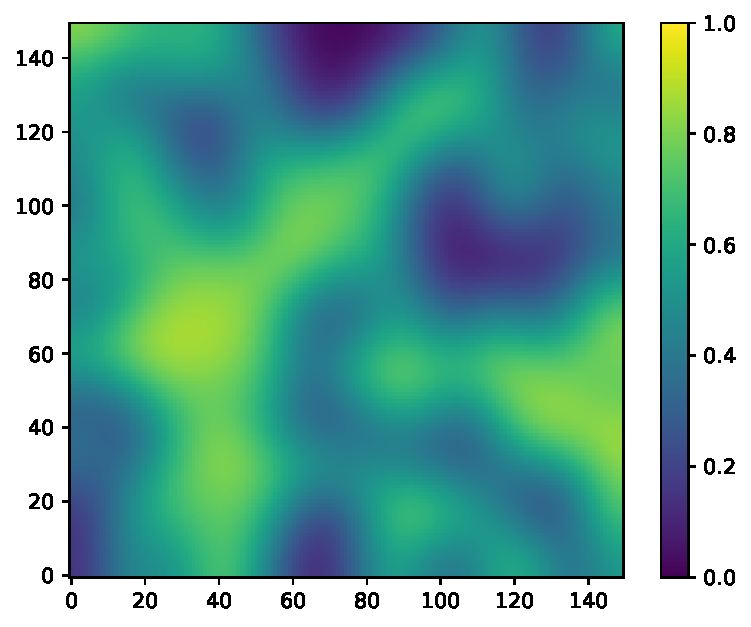
\includegraphics[height=2.5in]{figures/results/unblur/barkley_u_blur_blured.pdf}
		\setcapmargin[1cm]{1cm}
		\caption{Emuliertes Fernfeld}
		\label{fig:exp_unblur_barkley_blurred}
	\end{subfigure}%
	\begin{subfigure}{.5\textwidth}
		\centering
		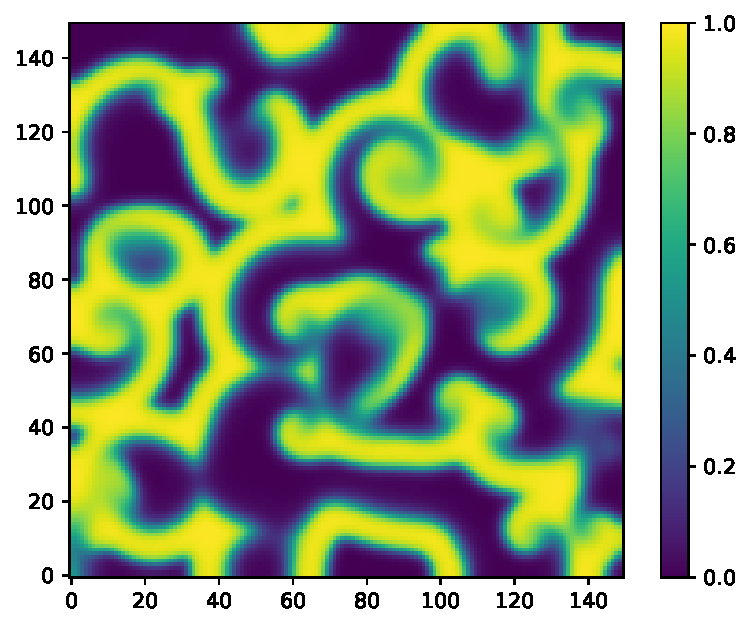
\includegraphics[height=2.5in]{figures/results/unblur/barkley_u_blur_orig.pdf}
		\setcapmargin[1cm]{1cm}
  		\caption{Echte Erregung des Modells}
  		\label{fig:exp_unblur_barkley_orig}
	\end{subfigure}
	\caption{Graphische Darstellung der $u$-Variable des \textit{Barkley}-Modells. Links ist das emulierte Fernfeld und rechts das tatsächliche $u$-Feld des Modells zu sehen.}
	\label{fig:exp_unblur_barkley}
\end{figure} 

\begin{figure}[h]
	\centering
	\begin{subfigure}{.5\textwidth}
		\centering
		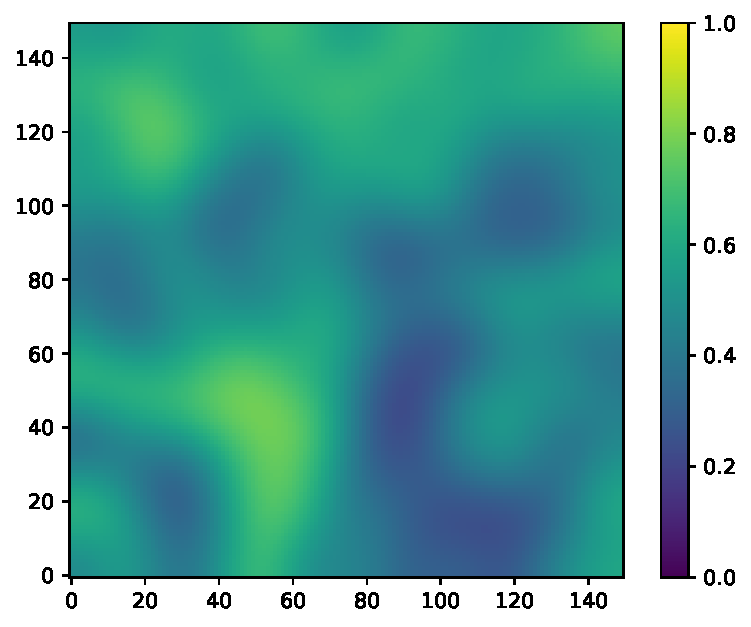
\includegraphics[height=2.5in]{figures/results/unblur/mitchell_v_blur_blured.pdf}
		\setcapmargin[1cm]{1cm}
		\caption{Emuliertes Fernfeld}
		\label{fig:exp_unblur_mitchell_schaeffer_blurred}
	\end{subfigure}%
	\begin{subfigure}{.5\textwidth}
		\centering
		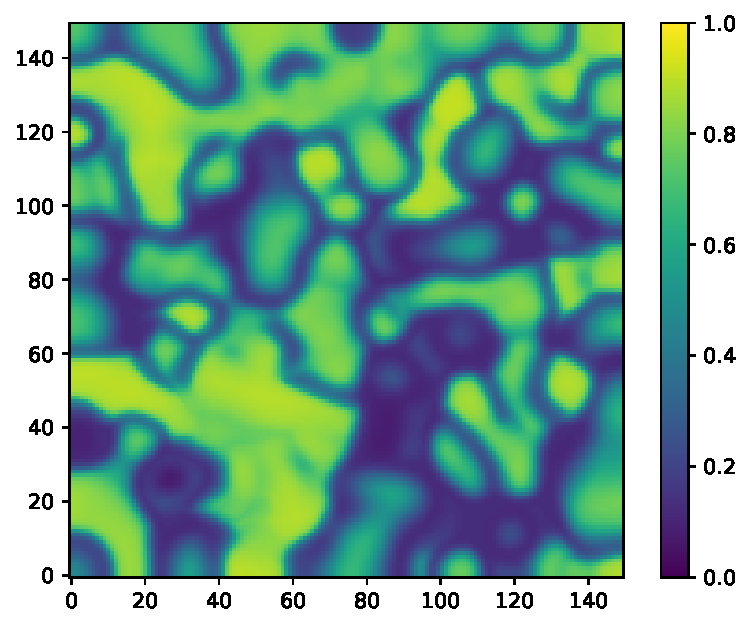
\includegraphics[height=2.5in]{figures/results/unblur/mitchell_v_blur_orig.pdf}
		\setcapmargin[1cm]{1cm}
  		\caption{Echte Erregung des Modells}
  		\label{fig:exp_unblur_mitchell_schaeffer_orig}
	\end{subfigure}
	\caption{Graphische Darstellung der $v$-Variable des \textit{Mitchell-Schaeffer}-Modells. Links ist das emulierte Fernfeld und rechts das tatsächliche $v$-Feld des Modells zu sehen.}
	\label{fig:exp_unblur_mitchell_schaeffer}
\end{figure} 

\subsection{Nächste Nachbar Vorhersage}
Zuerst wird diese Aufgabe erneut mit dem \textsc{NN}-Ansatz betrachtet. Die besten gefundenen Hyperparameter dafür sind in Tabelle \ref{tab:exp_unblur_nn_results} aufgelistet. Bemerkenswert ist erneut die geringe Laufzeit dieses Ansatzes. Dies wird durch die verhältnismäßig geringe Dimensionalität des Eingabe-Vektors begünstigt. Allerdings sind die Fehlerwerte sehr hoch, sodass die Vorhersage kaum besser ist, als eine Schätzung mit dem Mittelwert als Vorhersage.

\begin{table}[h]
	\centering

	\begin{tabular}{|c|c|c|}
		\multicolumn{1}{c|}{} & Barkley & Mitchell-Schaeffer \\ 
		\hline \hline 
		\rule[-1ex]{0pt}{2.5ex} $\sigma$ & $1$ & $1$ \\ 
		\hline 
		\rule[-1ex]{0pt}{2.5ex} $\Delta \sigma$ & $1$ & $1$ \\ 
		\hline 
		\rule[-1ex]{0pt}{2.5ex} $\delta$ & $4$ & $3$ \\ 
		\hline 
		\rule[-1ex]{0pt}{2.5ex} k & $5$ & $5$ \\ 
		\hline 
		\rule[-1ex]{0pt}{2.5ex} Laufzeit [s] & $53$ & $42$ \\ 
		\hline 
		\rule[-1ex]{0pt}{2.5ex} \textbf{MSE} & \textbf{0.10089} & \textbf{0.06217} \\ 
		\hline 
		\rule[-1ex]{0pt}{2.5ex} \textbf{NRMSE} & \textbf{0.8227} & \textbf{0.9136} \\ 
		\hline 
	\end{tabular} 

	\caption{Gefundene Hyperparameter der nächsten Nachbar Vorhersage für das \textit{Mitchell-Schaeffer}- und das \textit{Barkley}-Modell, welche zu den geringsten Fehlern führen.}
\label{tab:exp_unblur_nn_results}
\end{table} 


\FloatBarrier
\subsection{Radiale Basisfunktionen}
Als nächstes sind nun die radialen Basisfunktionen ebenfalls auf das Problem angewendet worden. Die dabei gefundenen Hyperparameter sind in Tabelle \ref{tab:exp_unblur_rbf_results} präsentiert.

\begin{table}[h]
	\centering

	\begin{tabular}{|c|c|c|}
		\multicolumn{1}{c|}{} & Barkley & Mitchell-Schaeffer \\ 
		\hline \hline 
		\rule[-1ex]{0pt}{2.5ex} $\sigma$ & $3$ & $5$ \\ 
		\hline 
		\rule[-1ex]{0pt}{2.5ex} $\Delta \sigma$ & $1$ & $2$ \\ 
		\hline 
		\rule[-1ex]{0pt}{2.5ex} $\delta$ & $3$ & $3$ \\ 
		\hline 
		\rule[-1ex]{0pt}{2.5ex} $\sigma_{RBF}$ & $5.0$ & $9.0$ \\ 
		\hline 
		\rule[-1ex]{0pt}{2.5ex} Laufzeit [s] & $1840$ & $1842$ \\ 
		\hline 
		\rule[-1ex]{0pt}{2.5ex} \textbf{MSE} & \textbf{0.03899} & \textbf{0.03252} \\ 
		\hline 
		\rule[-1ex]{0pt}{2.5ex} \textbf{NRMSE} & \textbf{0.5114} & \textbf{0.6913} \\ 
		\hline 
	\end{tabular} 
	\caption{Gefundene Hyperparameter der radialen Basisfunktionen für das \textit{Mitchell-Schaeffer}- und das \textit{Barkley}-Modell, welche zu den geringsten Fehlern führen.}
	\label{tab:exp_unblur_rbf_results}
\end{table} 


\FloatBarrier
\subsection{Echo State Network}
Nachdem die klassischen Methoden bereits auf dieses Problem angewendet worden sind, kann das Problem nun mittels der \textsc{ESN}s erneut betrachtet werden. Hierfür sind die verwendeten Hyperparameter erneut nach Abschnitt \ref{sec:exp_general_esn} gesucht worden. Die Ergebnisse sind in Tabelle \ref{tab:exp_unblur_esn_results} zu finden. Auffällig ist hierbei, dass die optimale Größe $N$ des Reservoirs für beiden Modelle unter der maximal betrachteten Größe $N \leq 400$ liegt. Dies kann ein Anzeichen dafür sein, dass für das Bewältigen der Aufgabe kein ausgeprägtes Langzeitgedächtnis vorhanden sein muss, da diese nach Abschnitt \ref{sc:esn} mit der Größe $N$ des Reservoirs skaliert. 
\improvement{Add more details on:long time memory vs N dependency in theory.}

\begin{table}[h]
	\centering
	\captionsetup{width=0.9\linewidth}
	\begin{tabular}{|c|c|c|}
		\multicolumn{1}{c|}{} &  Barkley & Mitchell-Schaeffer \\ 
		\hline \hline 
		\rule[-1ex]{0pt}{2.5ex} $\sigma$ & $7$ & $7$ \\ 
		\hline 
		\rule[-1ex]{0pt}{2.5ex} $\Delta \sigma$ & $1$ & $1$ \\ 
		\hline 
		\rule[-1ex]{0pt}{3.5ex} $N$ & $200$ & $50$ \\ 
		\hline 
		\rule[-1ex]{0pt}{3.5ex} $\rho(|\mathbf{W}|)$ & $1.50$ & $0.10$\\ 
		\hline 
		\rule[-1ex]{0pt}{3.5ex} $\alpha$ & $0.20$ & $0.05$ \\ 
		\hline 
		\rule[-1ex]{0pt}{3.5ex} $\epsilon$ & $0.1$ & $0.1$ \\ 
		\hline 
		\rule[-1ex]{0pt}{3.5ex} $\nu_{max}$ & $\num{1e-5}$ & $\num{1e-4}$\\ 
		\hline 
		\rule[-1ex]{0pt}{3.5ex} $\lambda$ & $\num{5e-10}$ & $\num{5e-6}$\\ 
		\hline 
		\rule[-1ex]{0pt}{2.5ex} Laufzeit [s] & $1603$ & $1540$ \\ 
		\hline 
		\rule[-1ex]{0pt}{2.5ex} \textbf{MSE} & \textbf{0.02347} & \textbf{0.02449} \\ 
		\hline
		\rule[-1ex]{0pt}{2.5ex} \textbf{NRMSE} & \textbf{0.3968} & \textbf{0.3599} \\ 
		\hline 
	\end{tabular} 
	\caption{Gefundene Hyperparameter des \textsc{ESN} für das \textit{Mitchell-Schaeffer}- und das \textit{Barkley}-Modell, welche zu den geringsten Fehlern führen.}
	\label{tab:exp_unblur_esn_results}
\end{table}

\FloatBarrier
\subsection{Vergleich}
Zusammenfassend können nun die Ergebnisse der drei Ansätze erneut verglichen werden. Eine vergleichende Übersicht ist in Tabelle \ref{tab:exp_unblur_esn_results} zu finden. Dort ist erneut zu bemerken, dass die \textsc{ESN}s die geringsten Fehlerwerte erzeugt, doch der \textsc{NN}-Ansatz deutlich schneller berechnet werden kann.\\
Zusätzlich zu der Tabelle ist noch ein exemplarischer grafischer Vergleich der Resultate der drei Ansätze mit dem Ziel in Abbildung \ref{fig:exp_unblur_barkley_result} dargestellt. Dort fällt auf, dass die Vorhersage des \textsc{NN}-Ansatzes selbst die Struktur der Dynamik kaum korrekt auflöst. Im Vergleich dazu ist die Vorhersage des \textsc{RBF}-Ansatzes und des \textsc{ESN} deutlich feiner und beinhaltet sogar die Makrostruktur der Dynamik. Des Weiteren ist zu bemerken, dass diese mit dem \textsc{ESN} leicht feiner aufgelöst worden ist, als mit \textsc{RBF}-Ansatz. Zwar stimmen hier auch nicht die feinen Details der Dynamik mit dem Original überein, doch ist eine starke Verbesserung im Vergleich zu dem emulierten Fernfeld zu bemerken. Unter Umständen wäre es für zukünftige Arbeiten bei dieser Aufgabe angebracht eine andere Fehlermetrik als die mittlere quadratische Abweichung zu benutzen, welche die Ähnlichkeit zwischen den Strukturen der Felder stärker berücksichtigt. 

\begin{figure}[h]
	\centering
	\begin{subfigure}{.5\textwidth}
		\centering
		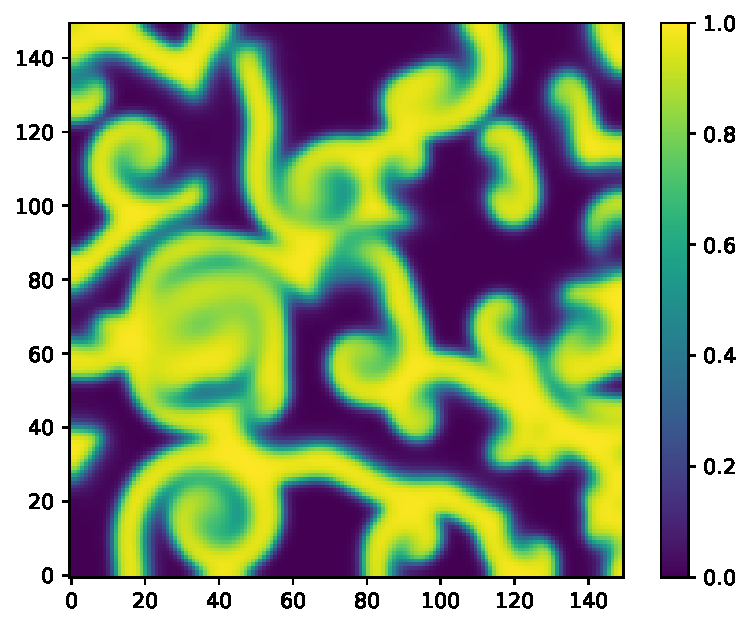
\includegraphics[height=2.5in]{figures/results/unblur/esn_barkley_u_blur_orig.pdf}
		\setcapmargin[1cm]{0.5cm}
		\caption{Echte Erregung des Modells}
		\label{fig:exp_unblur_barkley_result_orig}
	\end{subfigure}%
	\begin{subfigure}{.5\textwidth}
		\centering
		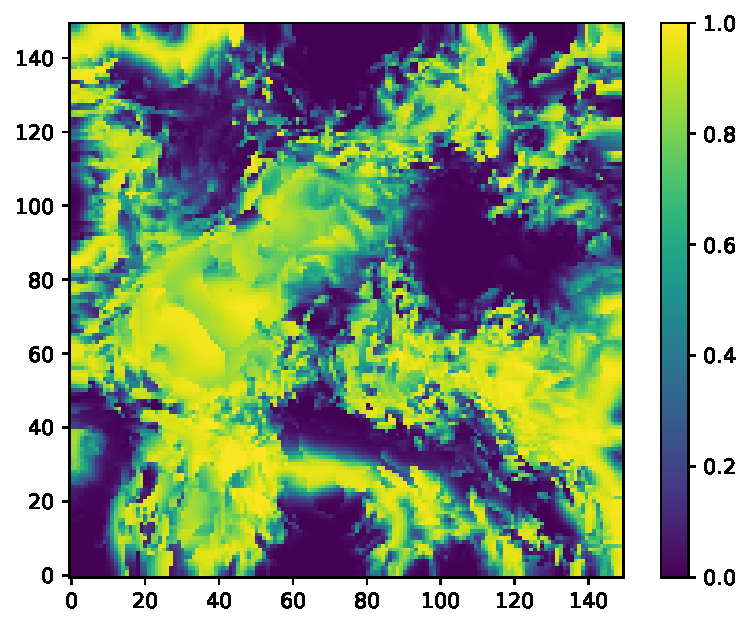
\includegraphics[height=2.5in]{figures/results/unblur/nn_barkley_u_blur_pred.pdf}
		\setcapmargin[1cm]{0.5cm}
  		\caption{Vorhersage des \textsc{NN}-Ansatzes}
  		\label{fig:exp_unblur_barkley_result_nn_pred}
	\end{subfigure}
	\begin{subfigure}{.5\textwidth}
		\centering
		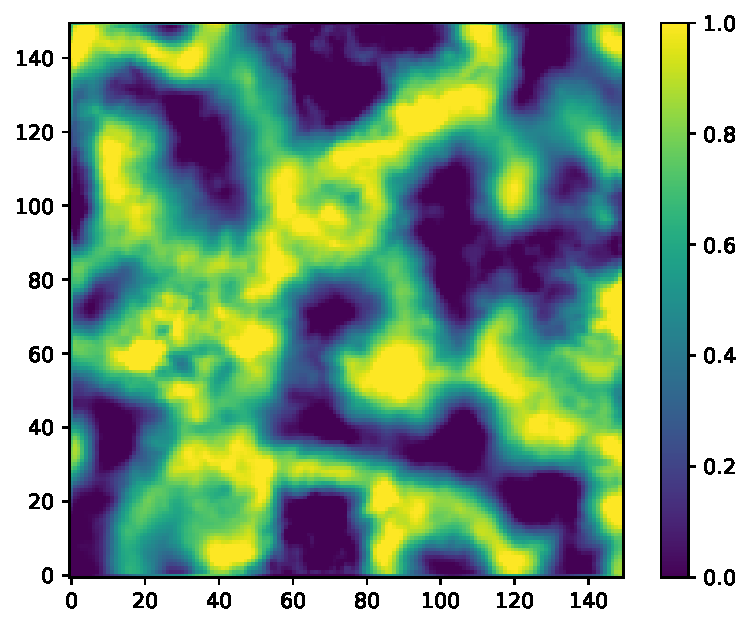
\includegraphics[height=2.5in]{figures/results/unblur/rbf_barkley_u_blur_pred.pdf}
		\setcapmargin[1cm]{0.5cm}
  		\caption{Vorhersage des \textsc{RBF}-Ansatzes}
  		\label{fig:exp_unblur_barkley_result_rbf_pred}
	\end{subfigure}%
	\begin{subfigure}{.5\textwidth}
		\centering
		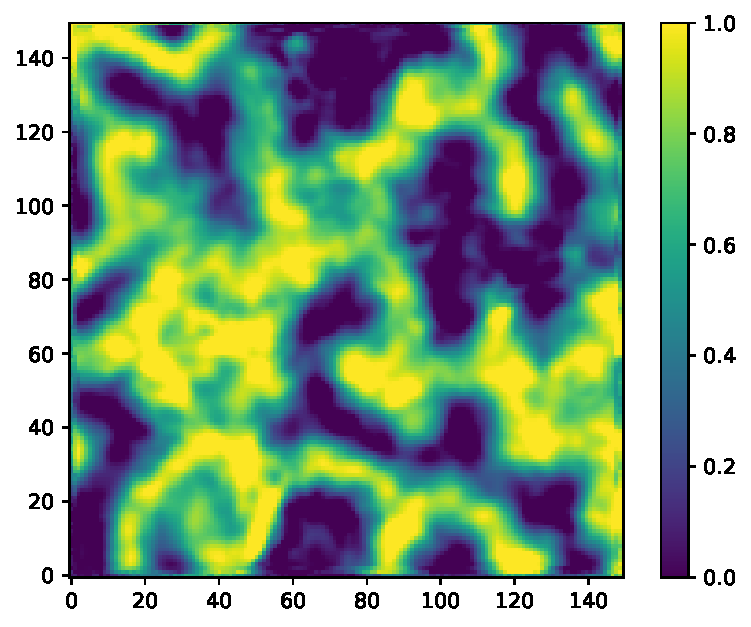
\includegraphics[height=2.5in]{figures/results/unblur/esn_barkley_u_blur_pred.pdf}
		\setcapmargin[1cm]{0.5cm}
  		\caption{Vorhersage des \textsc{ESN}}
  		\label{fig:exp_unblur_barkley_result_esn_pred}
	\end{subfigure}
	\caption{Graphische Darstellung der $u$-Variable des \textit{Barkley}-Modells für den $100$. Zeitschritt des Testdatensatzes. Oben links ist das tatsächliche Feld des Modells zu sehen. Danach folgenden im Uhrzeigersinn die Vorhersagen des \textsc{NN}-Ansatzes, des \textsc{RBF}-Ansatzes und des \textsc{ESN}.}
	\label{fig:exp_unblur_barkley_result}
\end{figure} 

\begin{table}[h]
	\centering
	\captionsetup{width=0.9\linewidth}
	\begin{tabular}{|c|c|c|c|c|c|c|c|}
		\multicolumn{1}{c|}{} & \multicolumn{3}{c|}{Barkley} & \multicolumn{3}{c|}{Mitchell-Schaeffer}		\\
		\cline{2-7}
		\multicolumn{1}{c|}{} & NN & RBF & ESN & NN & RBF & ESN \\
		
		\hline
		\hline
		
		Laufzeit [s] 	& \textbf{53} 	& 1840		& 3604				& \textbf{42}	& 1842 		& 3823 \\
		\hline
		MSE 			& 0.10089		& 0.03899	& \textbf{0.02347} 	& 0.06217		& 0.03252 	& \textbf{0.02449} \\
		\hline
		NRMSE 			& 0.8227		& 0.5114	& \textbf{0.3968} 	& 0.9136		& 0.6913 	& \textbf{0.3599} \\
		\hline 
	\end{tabular} 
	\caption{Vergleich der benötigten Laufzeit und der erreichten Fehlers der drei Ansätze für das \textit{Mitchell-Schaeffer}- und das \textit{Barkley}-Modell, welche zu den geringsten Fehlern führen.}
	\label{tab:exp_unblur_comparison_results}
\end{table}

\FloatBarrier